\subsubsection{Fakeable object definition tuning}

The main control region we use to measure the fake rate is enriched in QCD jet events, and is obtained selecting events with one loose lepton and an hadronic jet well separated from the lepton ($\Delta R> 0.7$).

For all muons and electrons with \pt above 30\GeV, events are selected at trigger level requiring a prescaled single lepton trigger (with no isolation requirements) and a particle flow jet with \pt 30\GeV reconstructed at HLT (40\GeV for low-\pt muons).
This implies that the fakeable objects in the measurement region all pass the lepton trigger, while in the application region this is not necessarily
the case, as we include also events triggered by a single or double lepton trigger.
In order to avoid a bias in the background estimate, we therefore need to have a definition of fakeable object so that the fake rate does not depend on
whether the lepton passes the trigger selection or not.

We assess this using non-prompt leptons in simulated lepton-enriched QCD events, where we can compare the fake rate with and without 
requiring the lepton to pass the trigger, for different choices of the fakeable object selection.
The study reveals two important features: first, the trigger turn-on imposes a cut on the reconstructed lepton \pt, and so it limits the amount of 
sideband available in the extrapolation for given bin in corrected lepton \pt. Because of this, a trigger with a given threshold, can only 
be used to measure the fake rate for significantly larger corrected \pt value, if we do not want the trigger theshold to bias the result.
For the definition used in this version of the analysis, the $\pt^{corr}/\pt \le 0.9/0.5=1.8$, so e.g. the HLT\_Mu8 trigger can be used starting from a corrected $\pt$ of $14.4\GeV$.
Because of these effects, we measure the fake rate for muons using a combination of the HLT\_Mu3\_PFJet40 trigger (for corrected $\pt \in [10,30]$\GeV), the HLT\_Mu8 trigger (for corrected $\pt \in [15, 45]$\GeV), an the HLT\_Mu17 trigger (for corrected $\pt$ above $30 \GeV$) and the HLT\_Mu27 trigger (for corrected $\pt$ above $45 \GeV$, after checking on the MC that there is no visible bias even if the trigger is fully efficieny only at corrected $\pt$ of about $48\GeV$); in the regions covered by multiple triggers, we combine them since the prescales are large and uncorrelated and thus the datasets are independent. For electrons, we use HLT\_EleX\_CaloIdM\_TrackIdM\_PFJet30 triggers, with thresholds of $8 \GeV$ (for $\pt \in [15,20]\GeV$), $12 \GeV$ (for $\pt \in [20,30]\GeV$), and $17 \GeV$ (for $\pt > 30\GeV$)

Beyond the impact of the \pt threshold, the trigger can also bias the fake rate if it has requirements in identification or isolation that are not strictly looser 
than the selection used at the denominator. For muons, as long as we use triggers with no isolation requirements this is not the case. In the case of electrons, the identification criteria applied at HLT, cut-based, are different from those offline (mva-based), and so we would have a mismatch even for electrons well above the \pt threshold of the trigger.

We solve this by tightening the electron fakeable object definition including in it also some cut-based electron identification criteria. The selection criteria to emulate the trigger are chosen by comparing electron identification variables for non-prompt electrons in QCD MC events for electrons that pass or fail the trigger. The cuts have to be tight enough that for events passing them the fake rate does not depend strongly on whether the event passes or fails the trigger. However, cuts need to be not too tight less they start causing a loss of signal efficiency, because they use the identification variables in a less optimal way than the mva electron identification. For the criteria we use in this analysis, the loss of efficiency introduced by these cuts for signal MC events that pass the full analysis selection and trigger is about $3\%$ in both the dielectron and electron-muon final states. In this version of the analysis, we apply these additional criteria on electrons irrespectively of their $\pt$, while in older versions of the analysis the request was relaxed for corrected $\pt < 30\GeV$.  
\begin{figure}[htb]
	\centering 
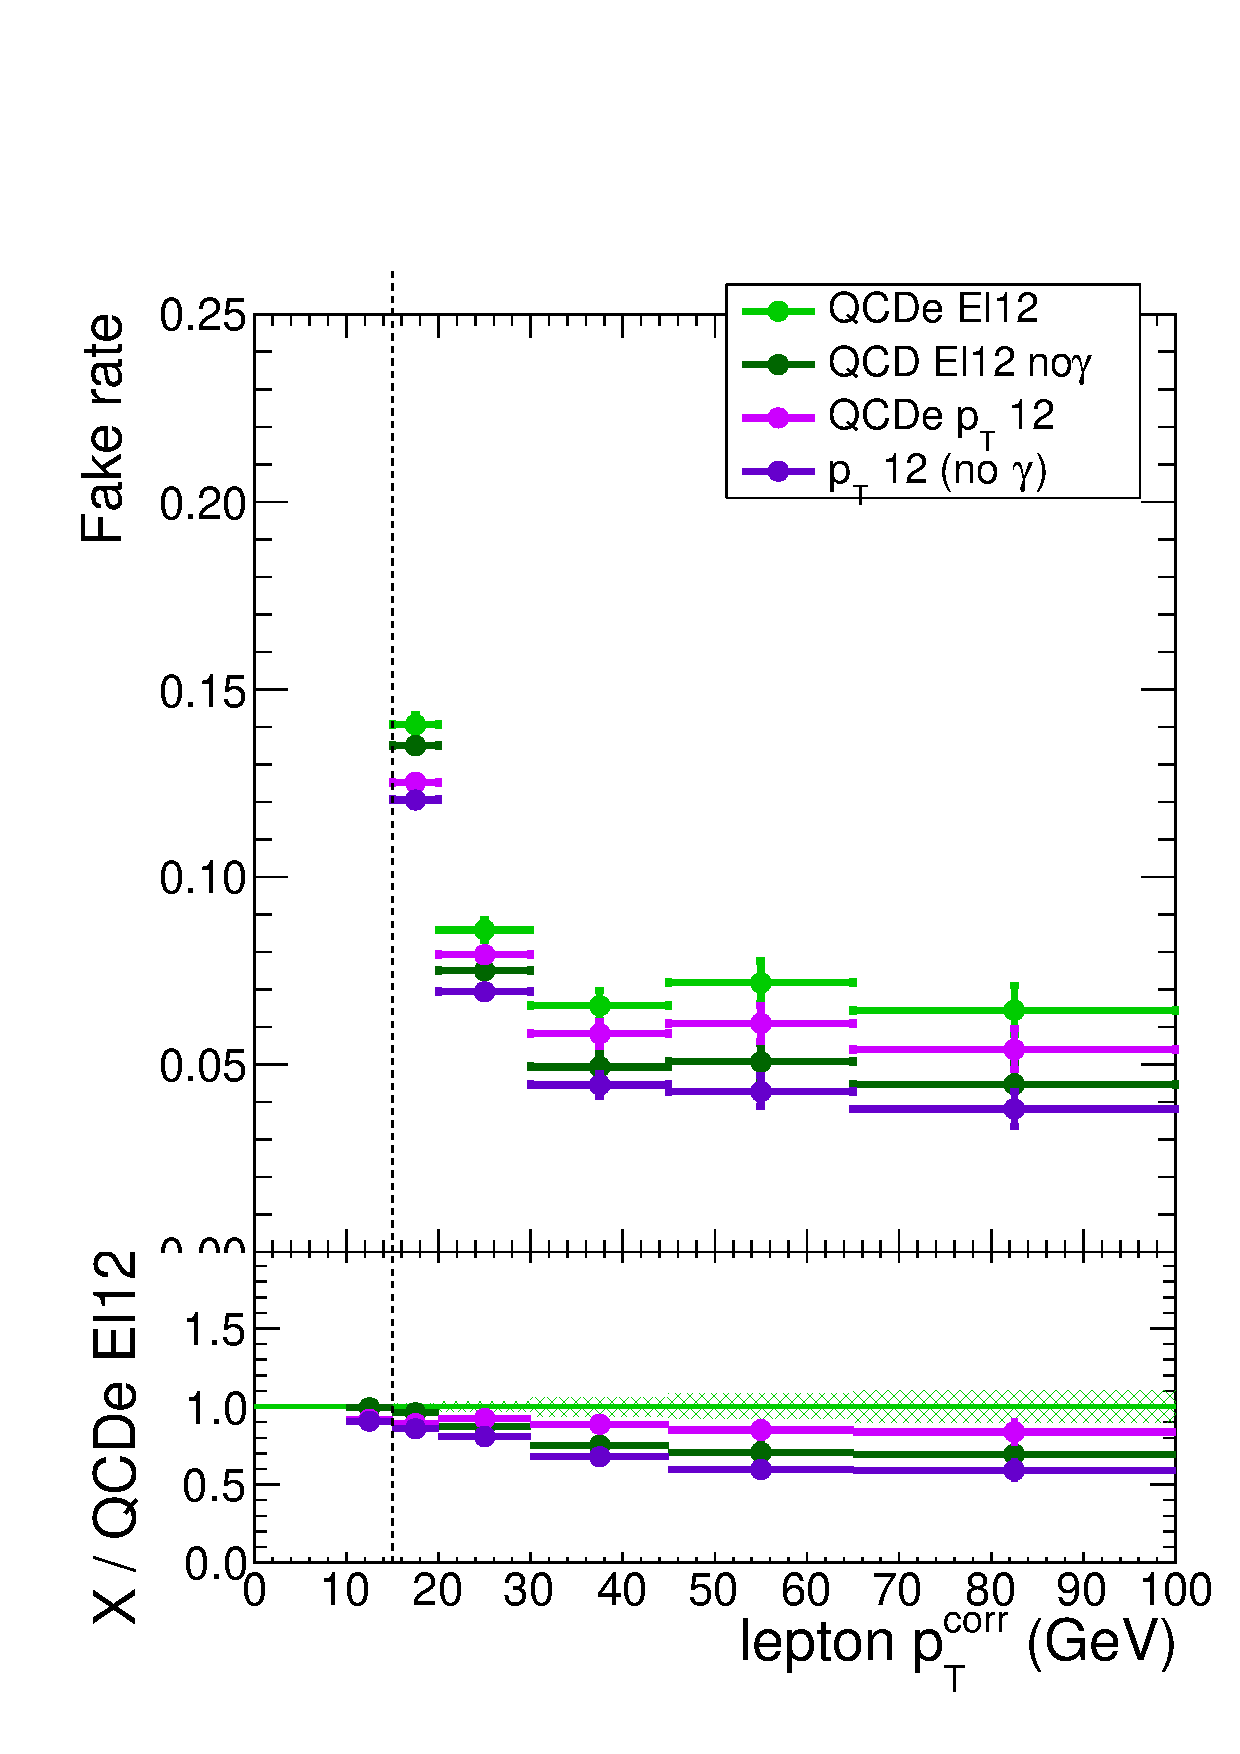
\includegraphics[width=0.35\textwidth]{plots_fakerate/measurement/el_hltid_barrel}
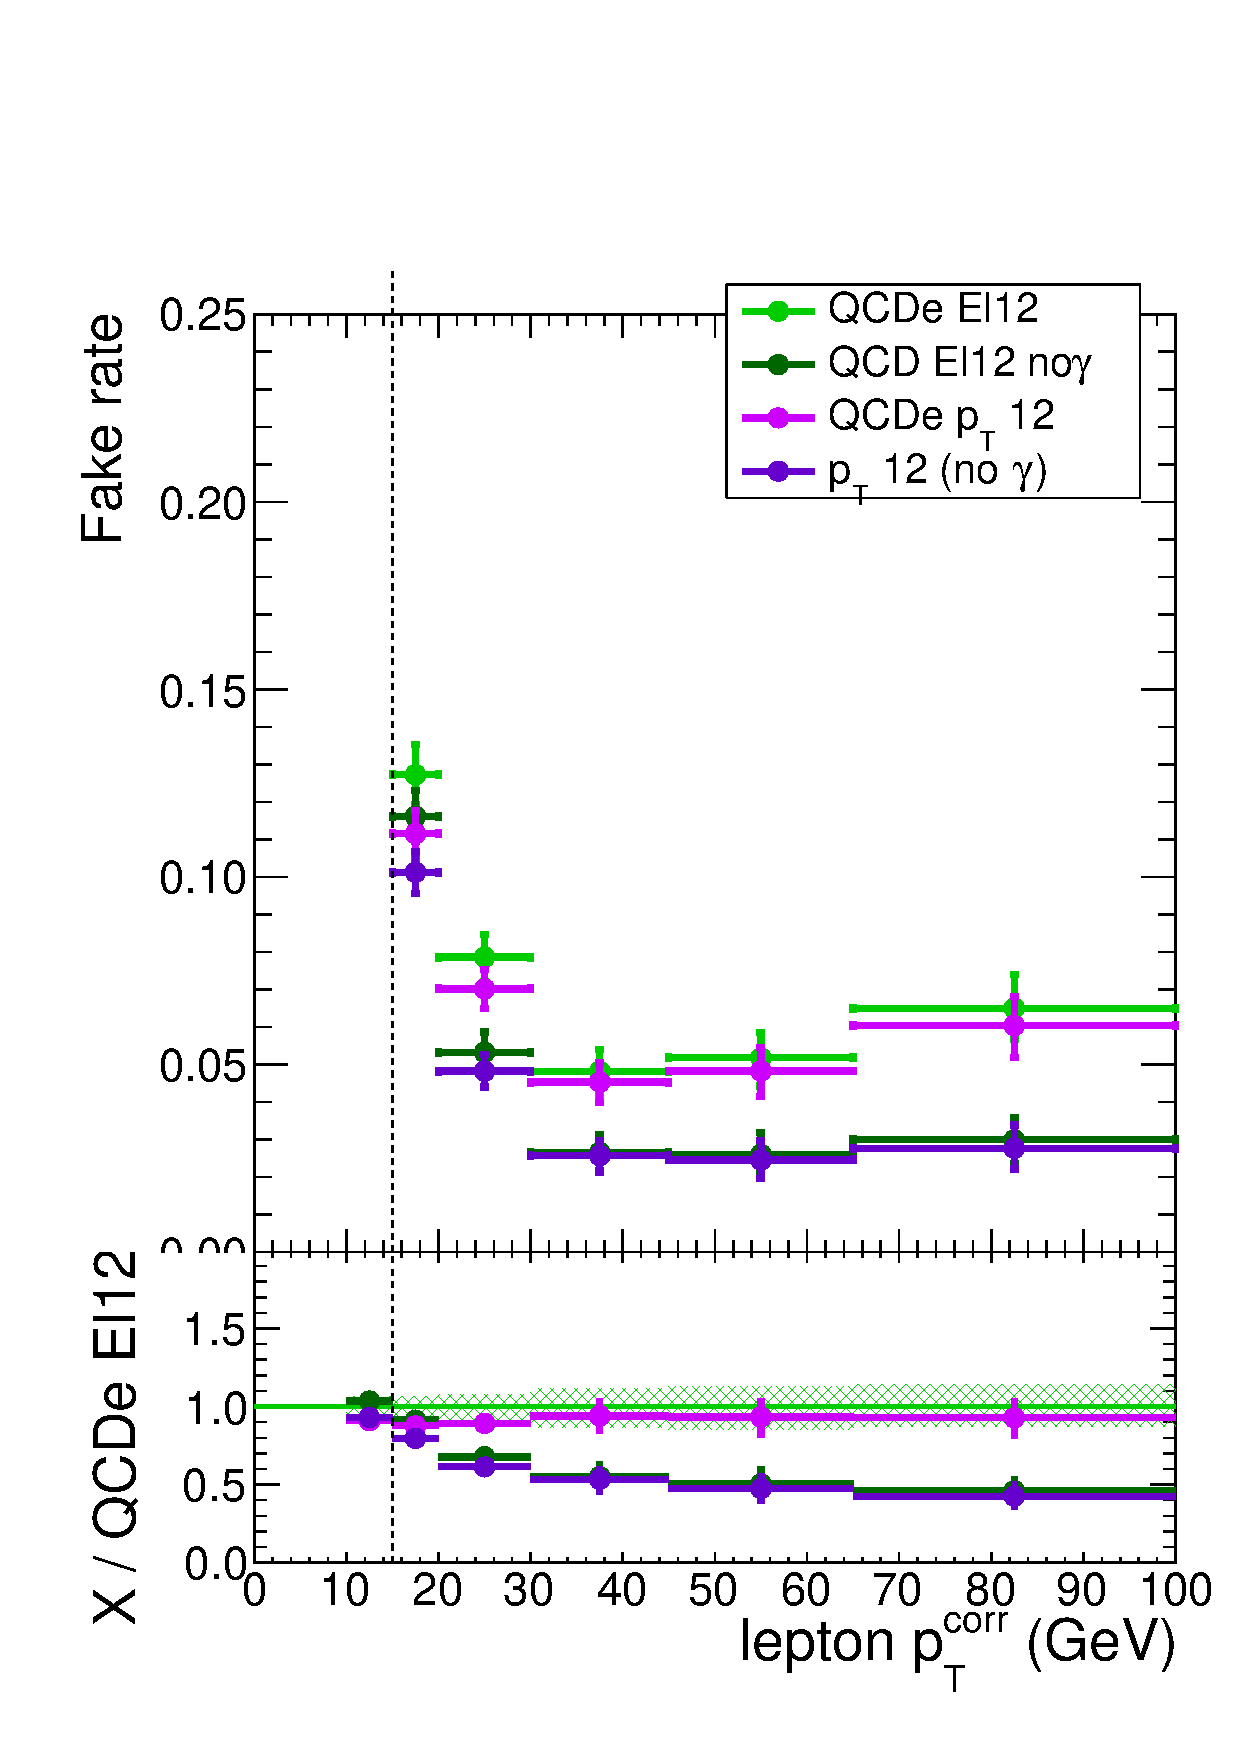
\includegraphics[width=0.35\textwidth]{plots_fakerate/measurement/el_hltid_endcap}
	\caption{Fake rate for electrons in the barrel (left) and endcaps (right) from simulated QCD multi-jet events, before the trigger requirement (pink) and after (green). The lighter shades of pink and green are  for all reconstructed electrons in the sample, while the darker shades are excluding the electrons that originate from the conversions of prompt photons (i.e. photons not hadron decays).} 
	\label{fig:frmeas-hltid}
\end{figure}


The choice of the lepton identification criteria on the fakeable object determine, together with the working point used for the tight lepton definition, the the fake rate for fake leptons, while they do not affect substantially the fake rate for non-prompt leptons originating from the decay of heavy flavour hadrons. On the other hand, the cut on the b-tagging discriminator of the jet associated to the lepton in the fakeable object definition can alter the fake rate for non-prompt leptons from heavy flavour without affecting fake leptons which are mostly originating from light jets. Thus, we can tune this cut to make the two fake rates more similar, and thus reduce the uncertainties associated to the flavour dependency of the fake rate. The quality of the tuning can be evaluated comparing e.g. the fake rates in $\ttbar$ events in the application region for the b-loose and b-tight category, that have different flavour compositions (Fig.~\ref{fig:frmeas-closure-ttvars}).
\begin{figure}[htb]
	\centering 
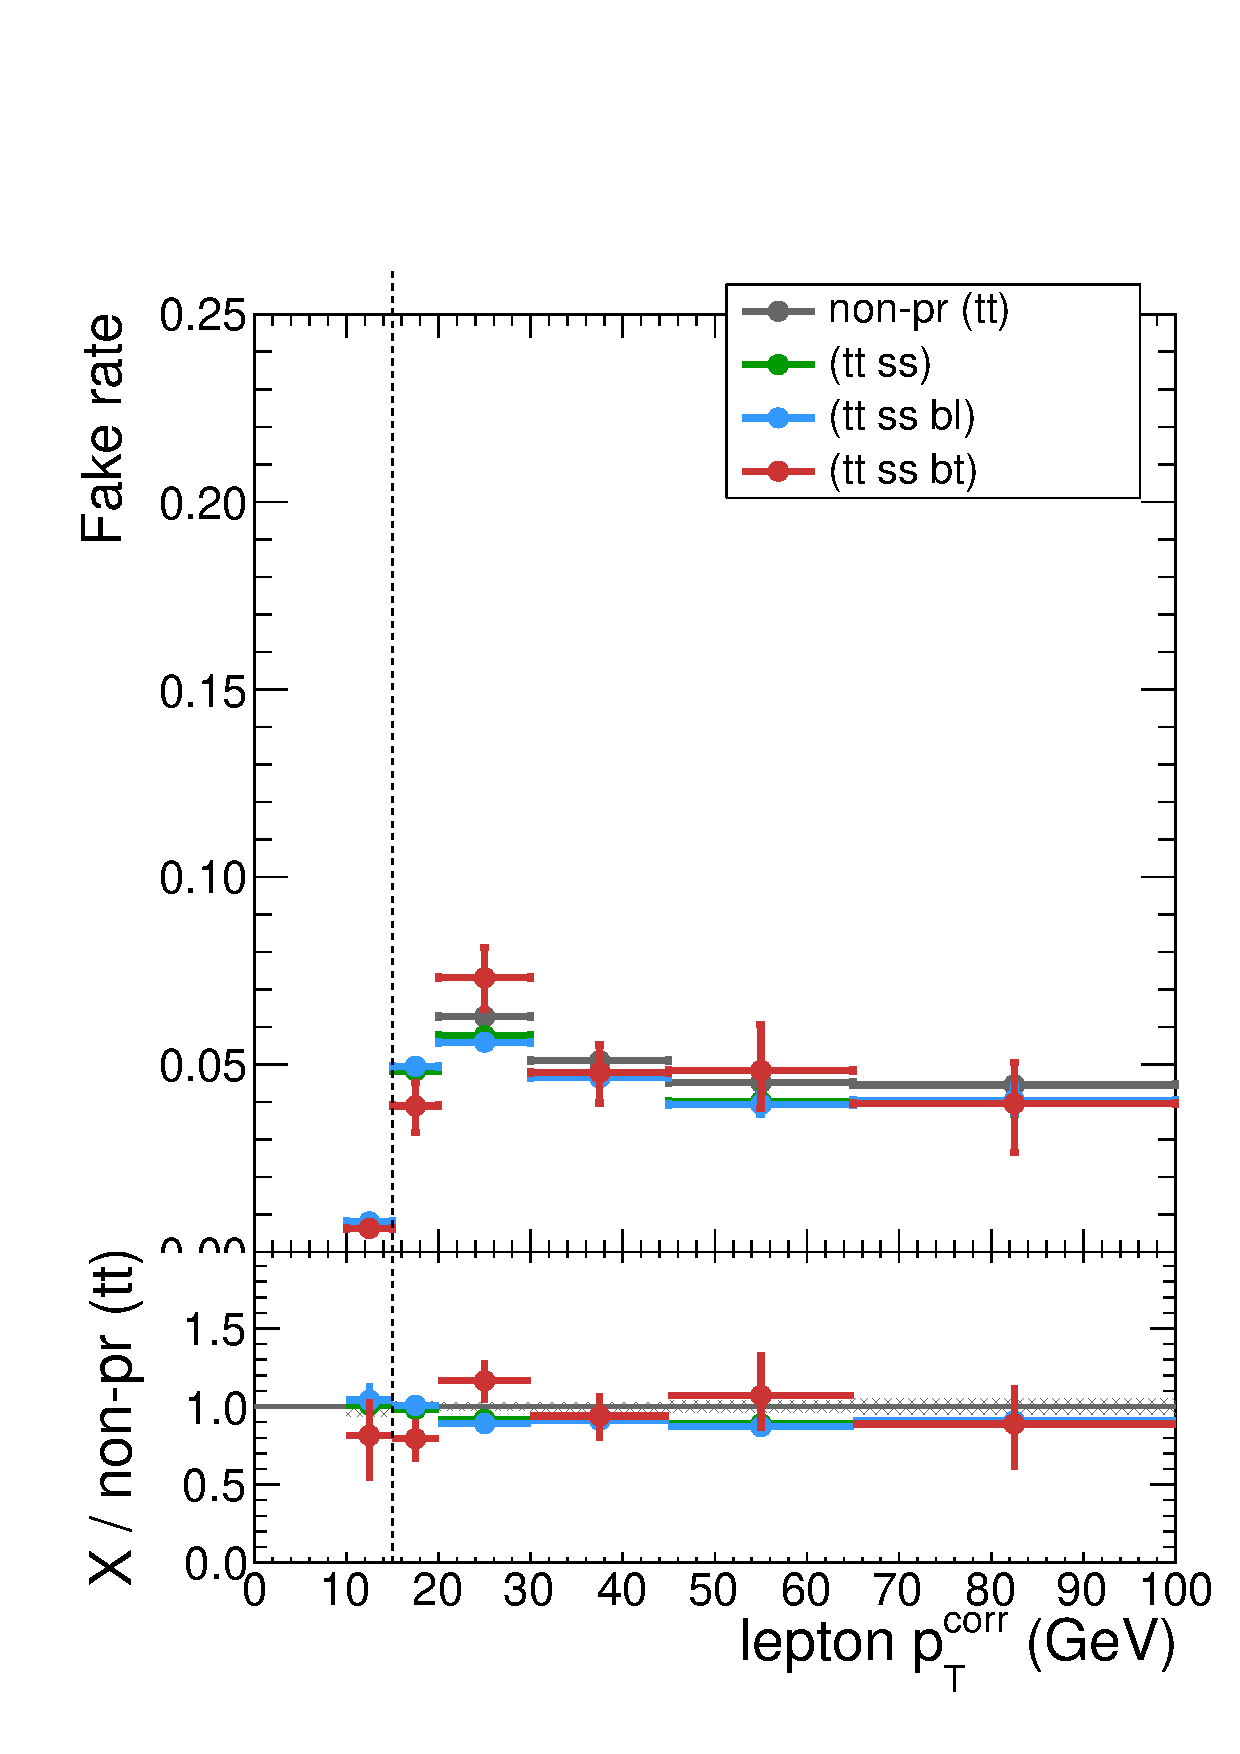
\includegraphics[width=0.35\textwidth]{plots_fakerate/measurement/mu_ttvars_barrel}
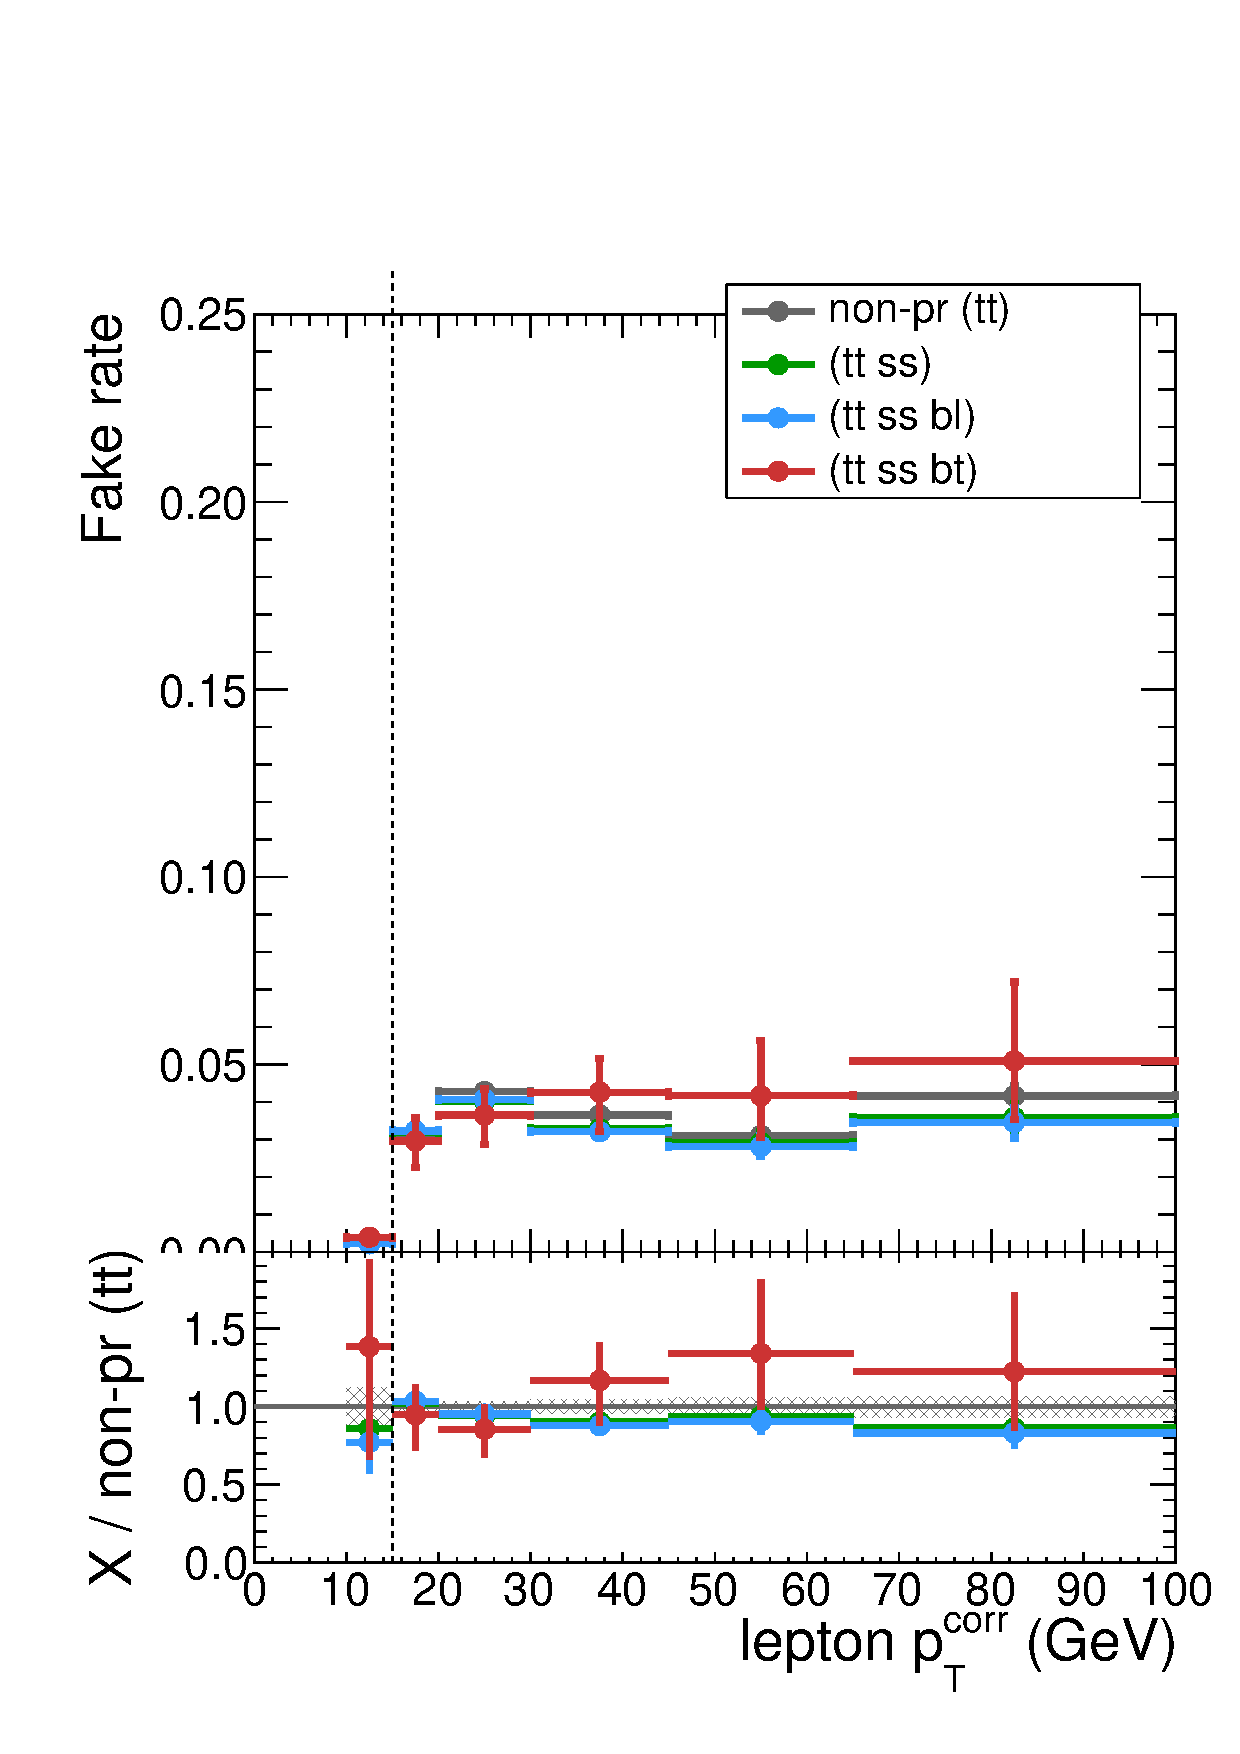
\includegraphics[width=0.35\textwidth]{plots_fakerate/measurement/mu_ttvars_endcap} \\
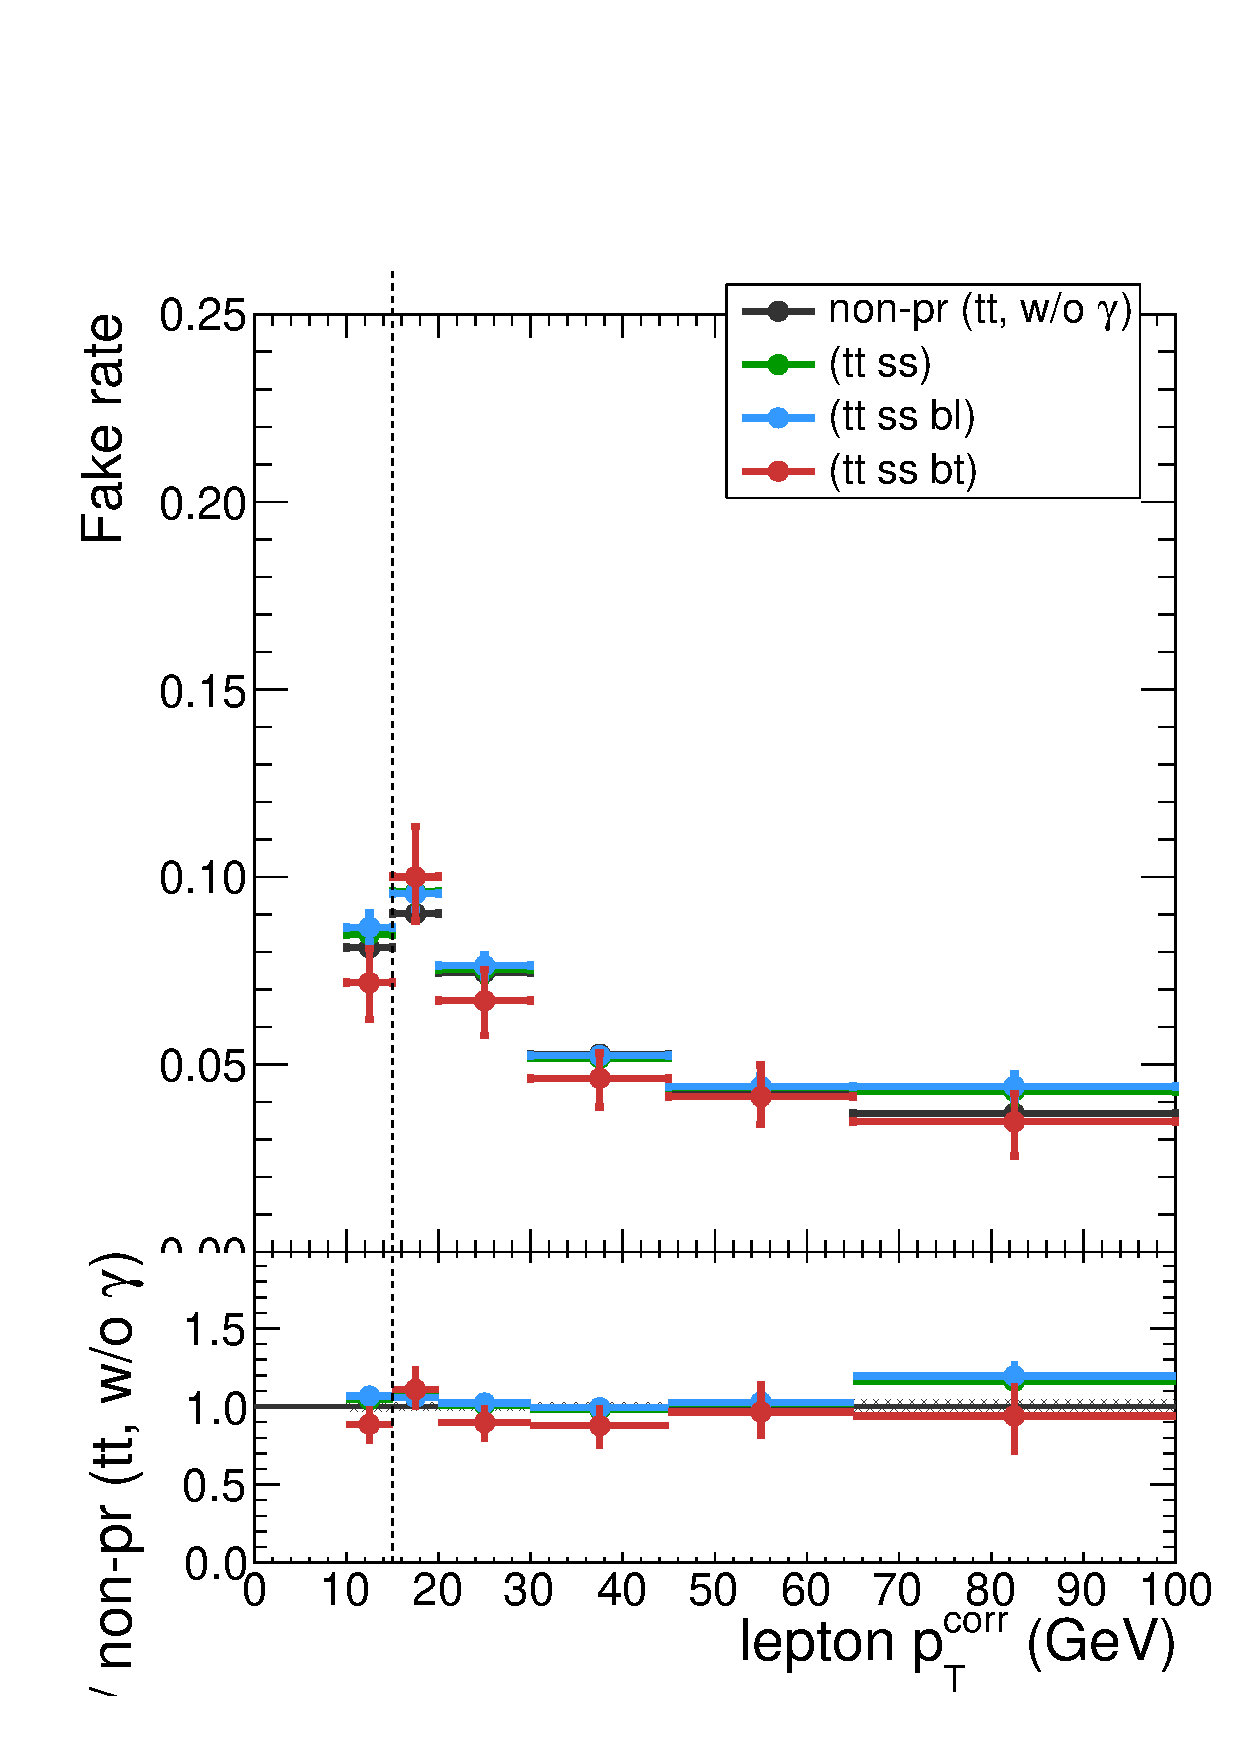
\includegraphics[width=0.35\textwidth]{plots_fakerate/measurement/el_ttvarsNC_barrel}
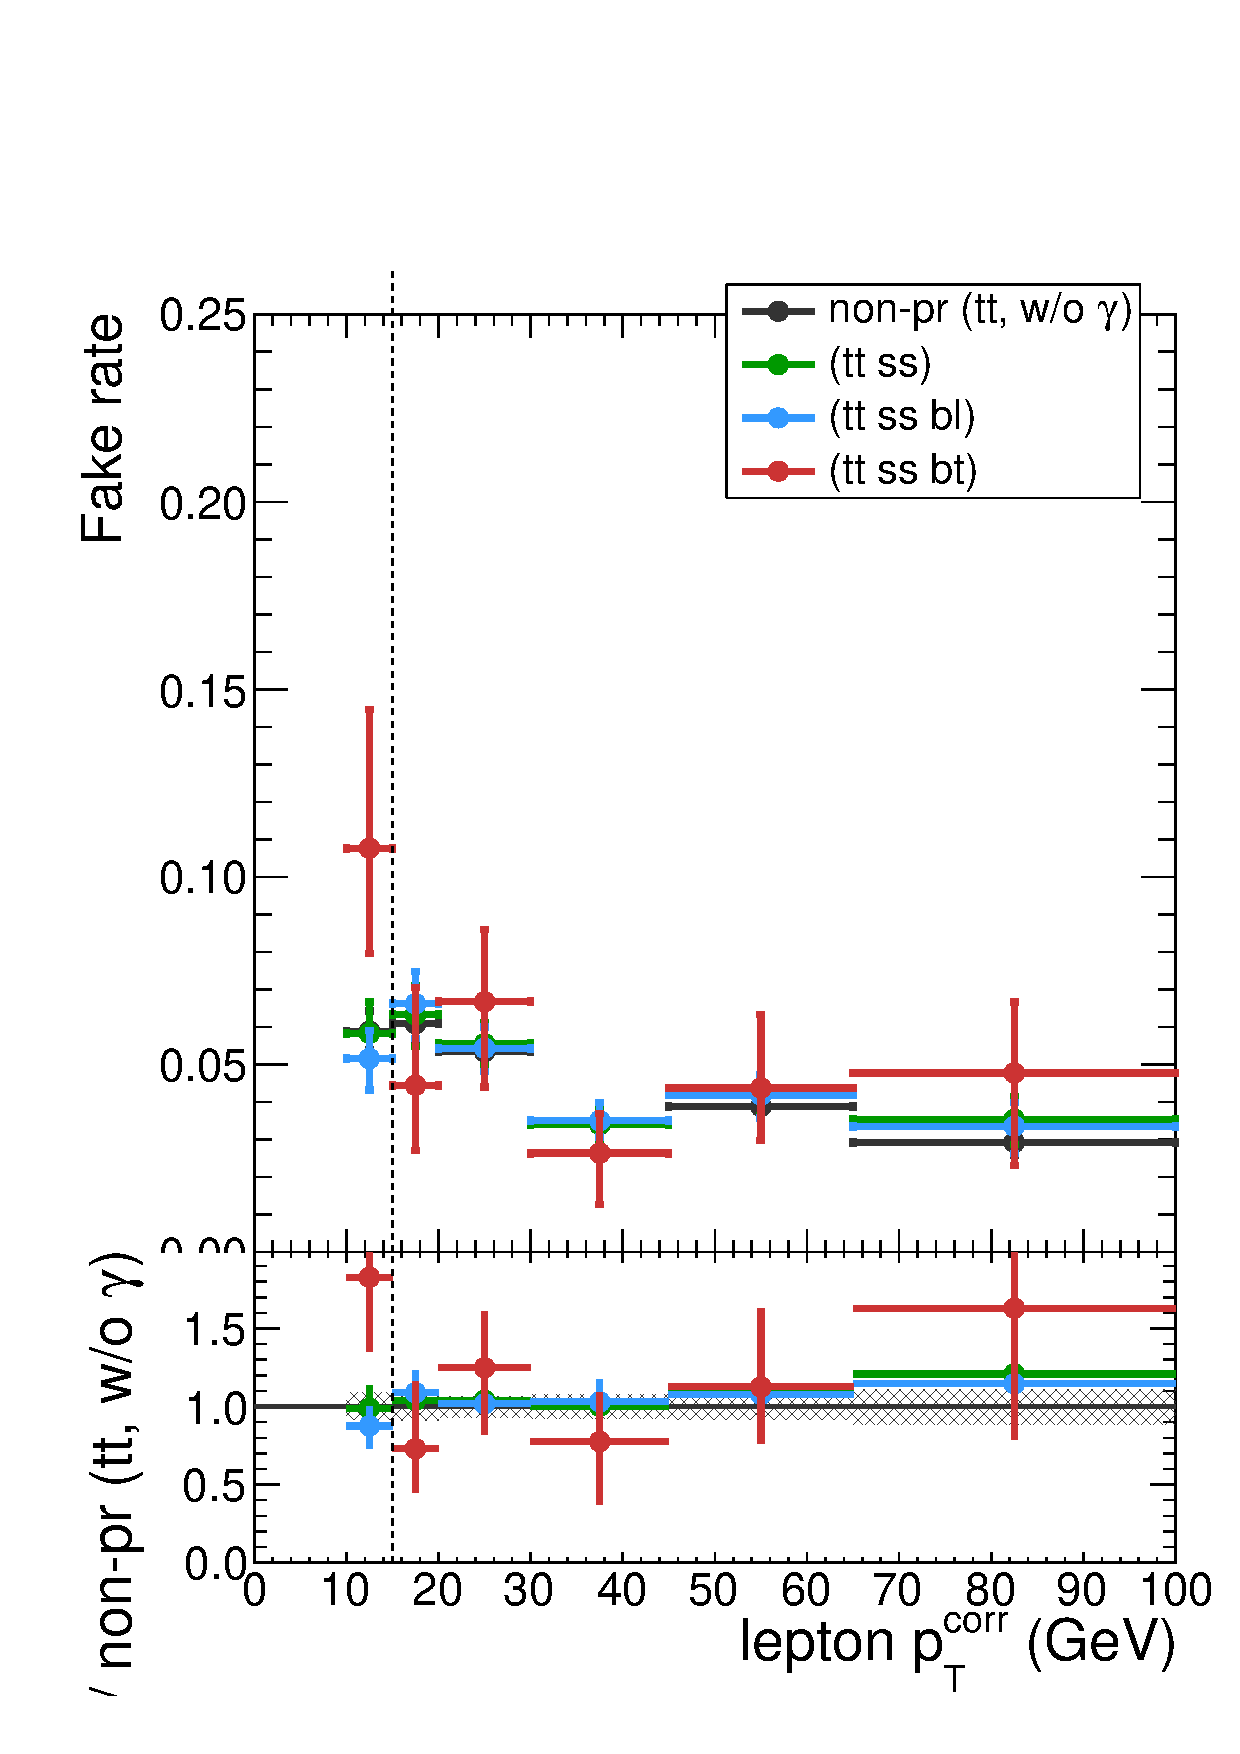
\includegraphics[width=0.35\textwidth]{plots_fakerate/measurement/el_ttvarsNC_endcap}
	\caption{Fake rate for muons (top) and electrons (bottom) in the barrel (left) and endcaps (right), from simulated $\ttbar$ events, inclusively (gray), in same-sign events (green), in same-sign events in the b-loose category (blue), and in same sign-events in the b-tight category (red). Electrons originating from the conversion of prompt photons are excluded from the plots.}
	\label{fig:frmeas-closure-ttvars}
\end{figure}


\subsubsection{QCD measurement region definition cuts}
For a fixed choice of the fakeable object and numerator, we can then assess how the fake in QCD events agrees with that of $\ttbar$, and how it depends on the cuts on the tag jet used to select the events.
A comparison of fake rates for background muons in $\ttbar$ and QCD is shown in Fig.~\ref{fig:frmeas-closure-bnb-mu}, both inclusively and selecting only leptons from b-jets. Overall, QCD and ttbar are found to agree to better than $20\%$.  For the central value of the measurement, for corrected $\pt < 30 \GeV$ we require one loose b-tagged jet away from the lepton, while we at higher $\pt$ we drop this requirement.
\begin{figure}[htb]
	\centering 
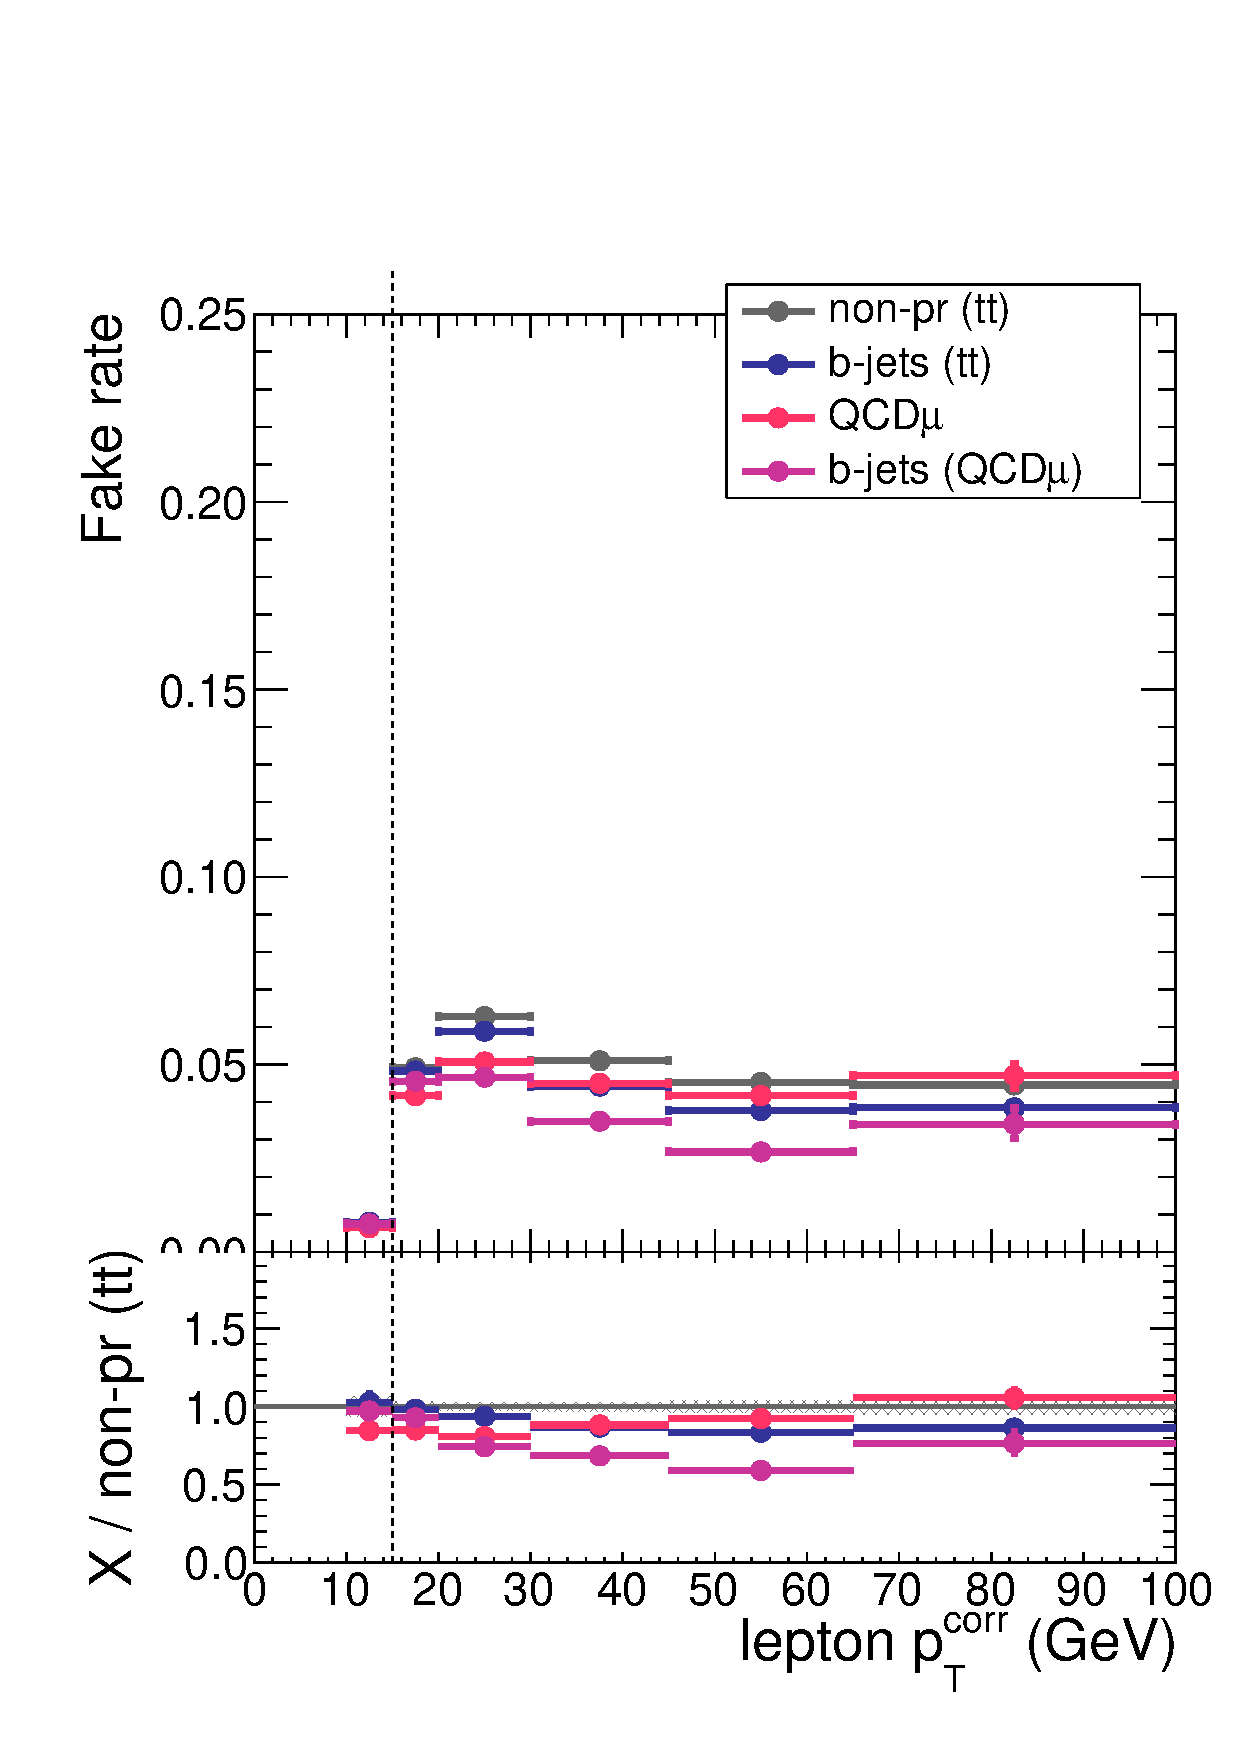
\includegraphics[width=0.35\textwidth]{plots_fakerate/measurement/mu_bnb_barrel}
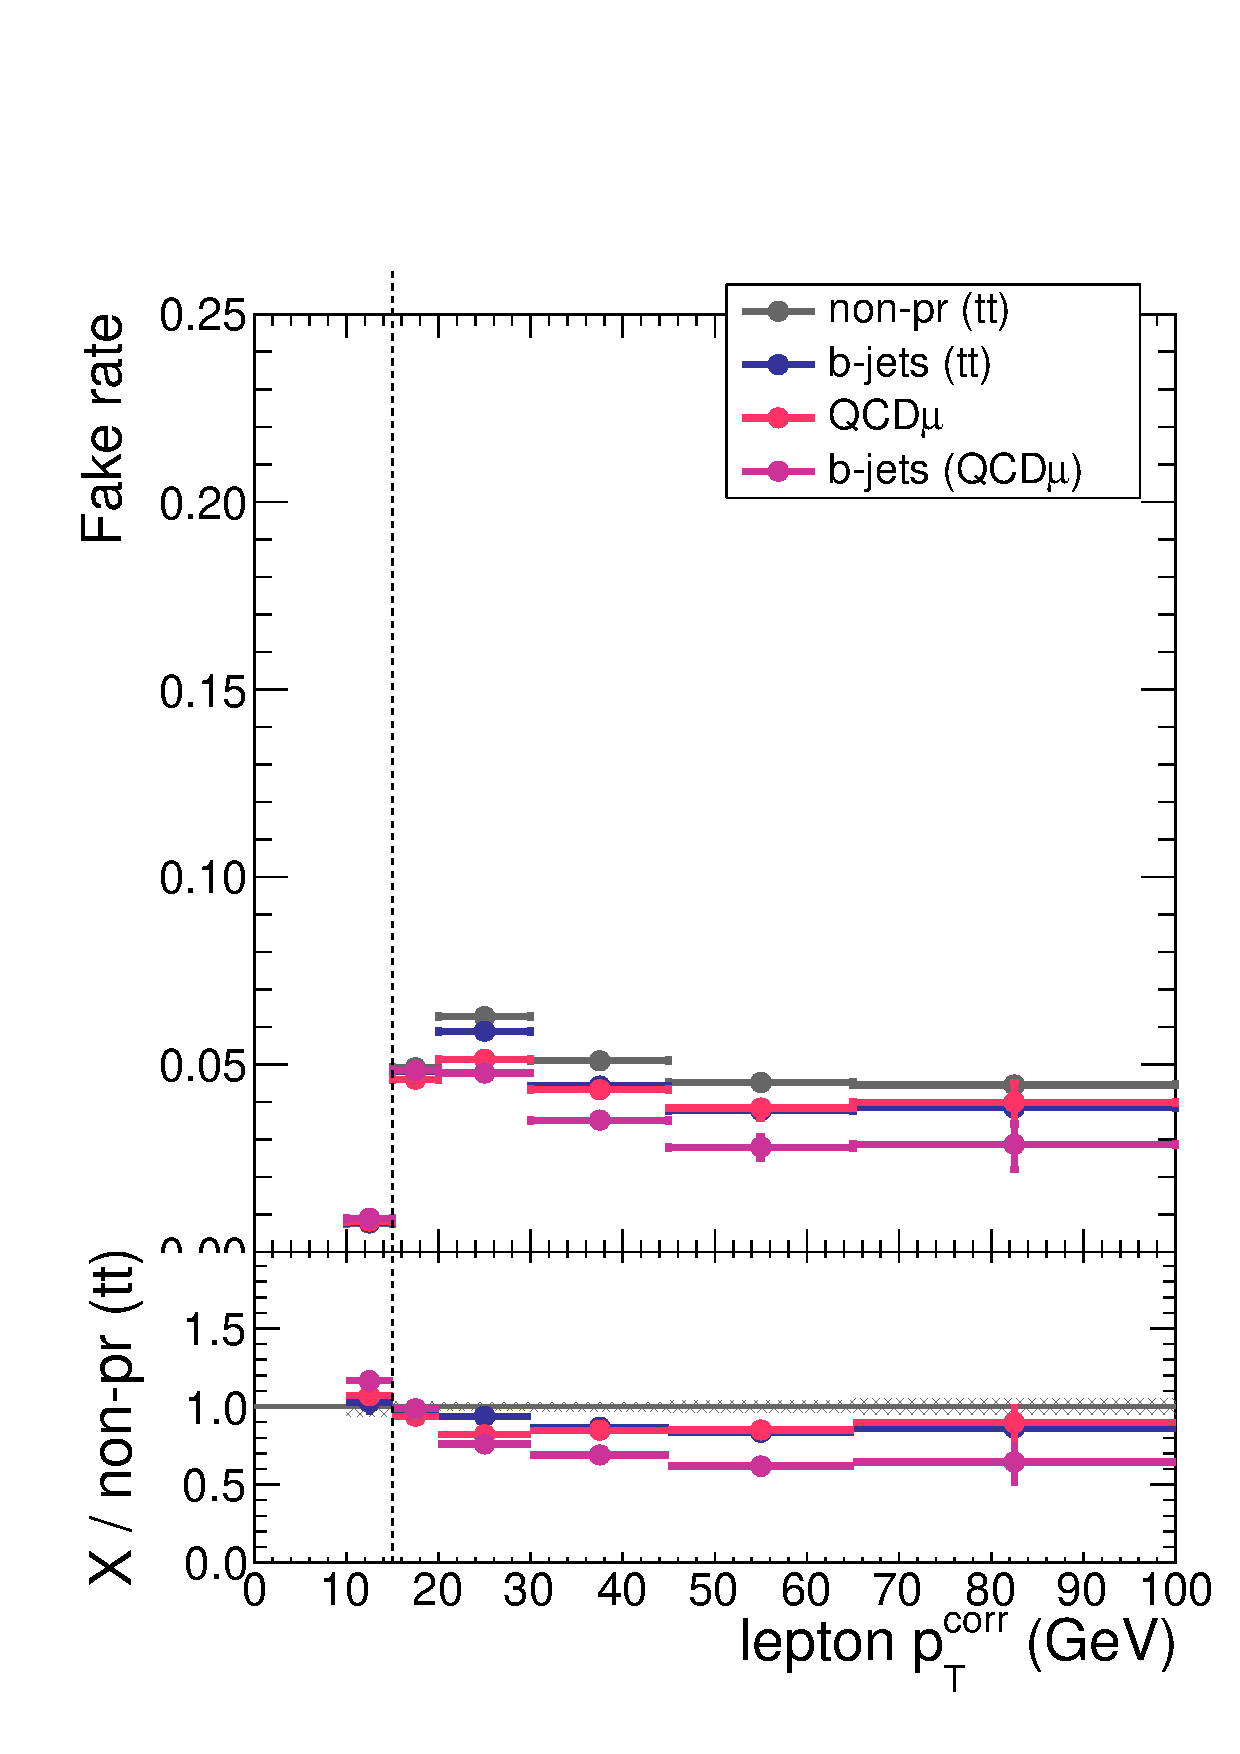
\includegraphics[width=0.35\textwidth]{plots_fakerate/measurement/mu_bnb_barrel_oneLoose}
	\caption{Fake rate for background muons in the barrel, from simulated $\ttbar$ and QCD events, inclusively or selecting only those from B hadron decays. The plot on the left is requiring only one away jet of $\pt > 30\GeV$, while the one on the right additionally require one loose b-tag.}
	\label{fig:frmeas-closure-bnb-mu}
\end{figure}

A comparison of fake rates for background electrons in $\ttbar$ and QCD is shown in Fig.~\ref{fig:frmeas-closure-bnb-el}. The agreement is excellent in the barrel at low and moderate $\pt$, and in general within $20\%$ everywhere. Electrons from conversions are a sizeable contribution to the fake rate especially in the endcaps and at high $\pt$.
\begin{figure}[htb]
	\centering 
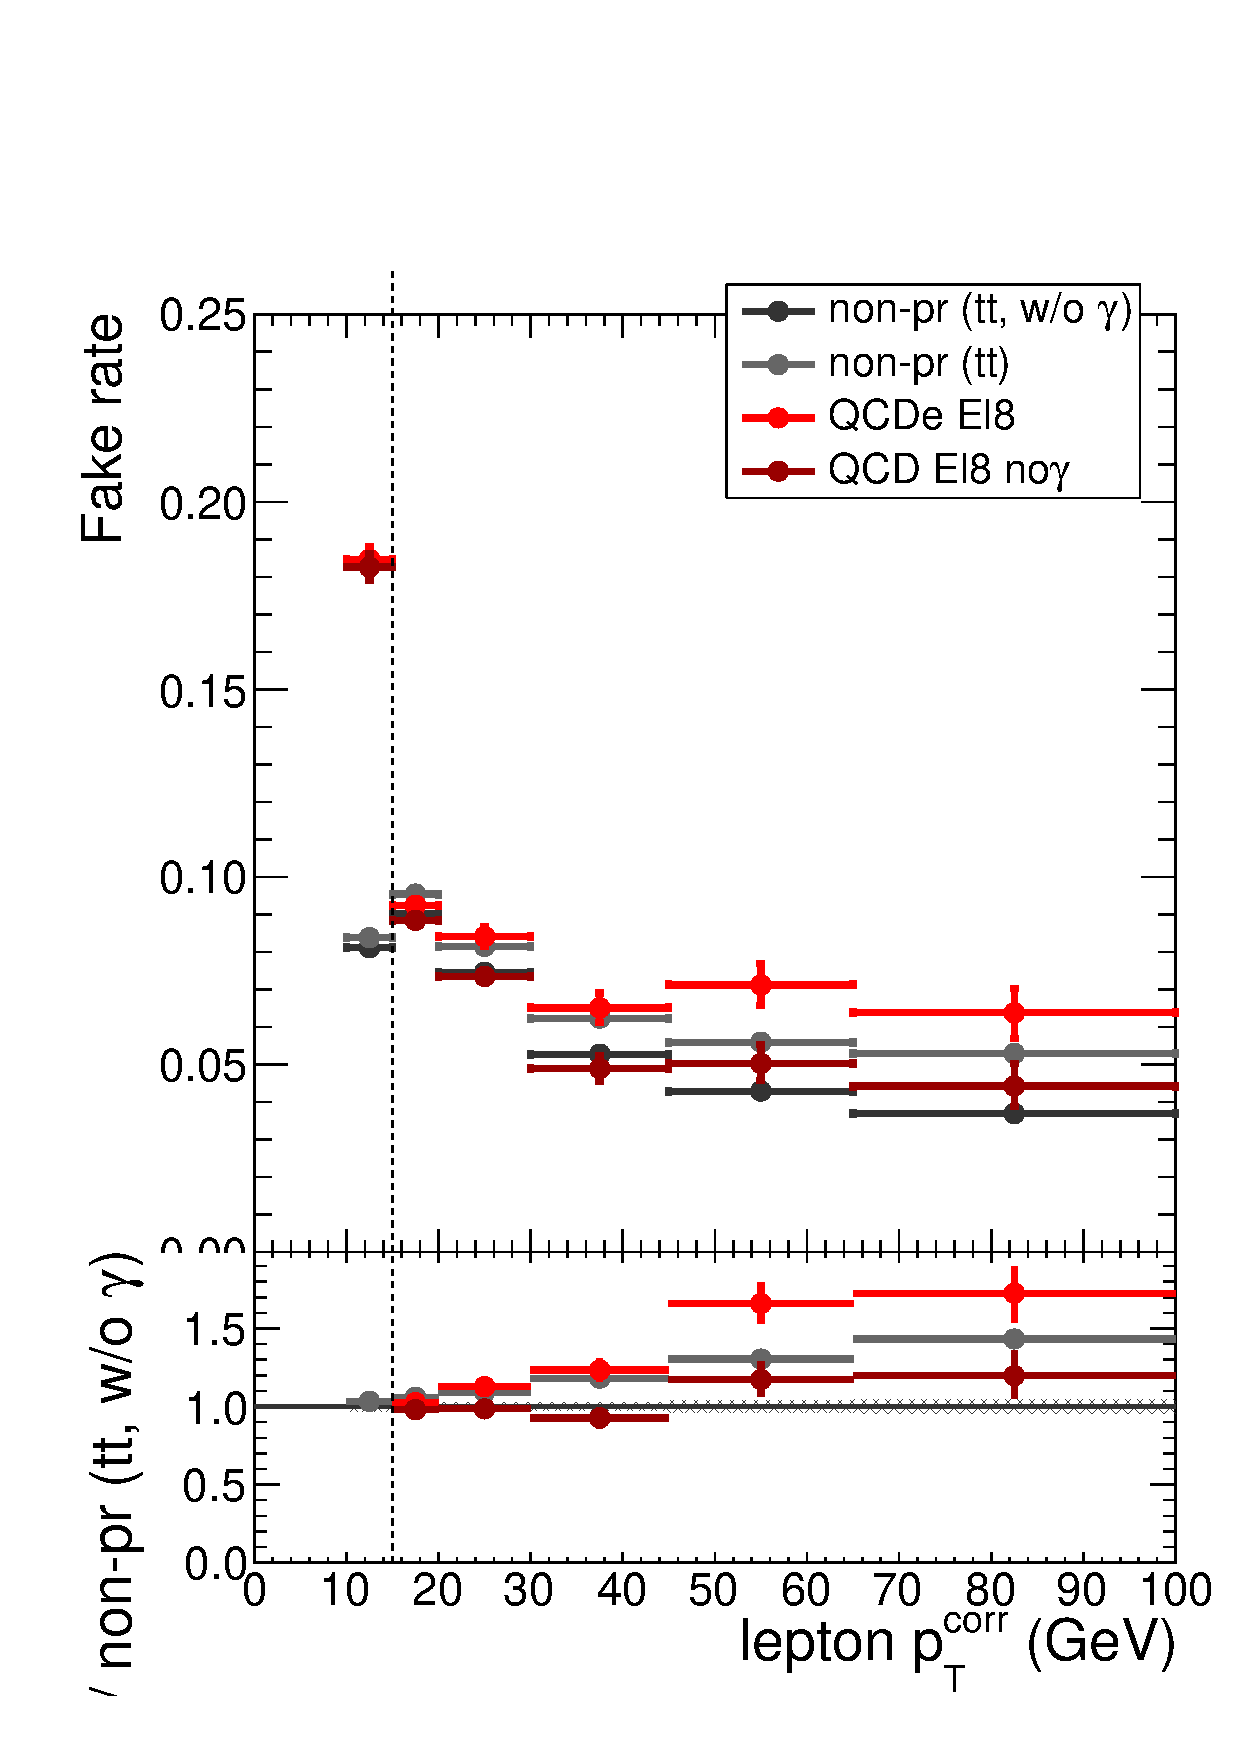
\includegraphics[width=0.35\textwidth]{plots_fakerate/measurement/el_lbin_barrel}
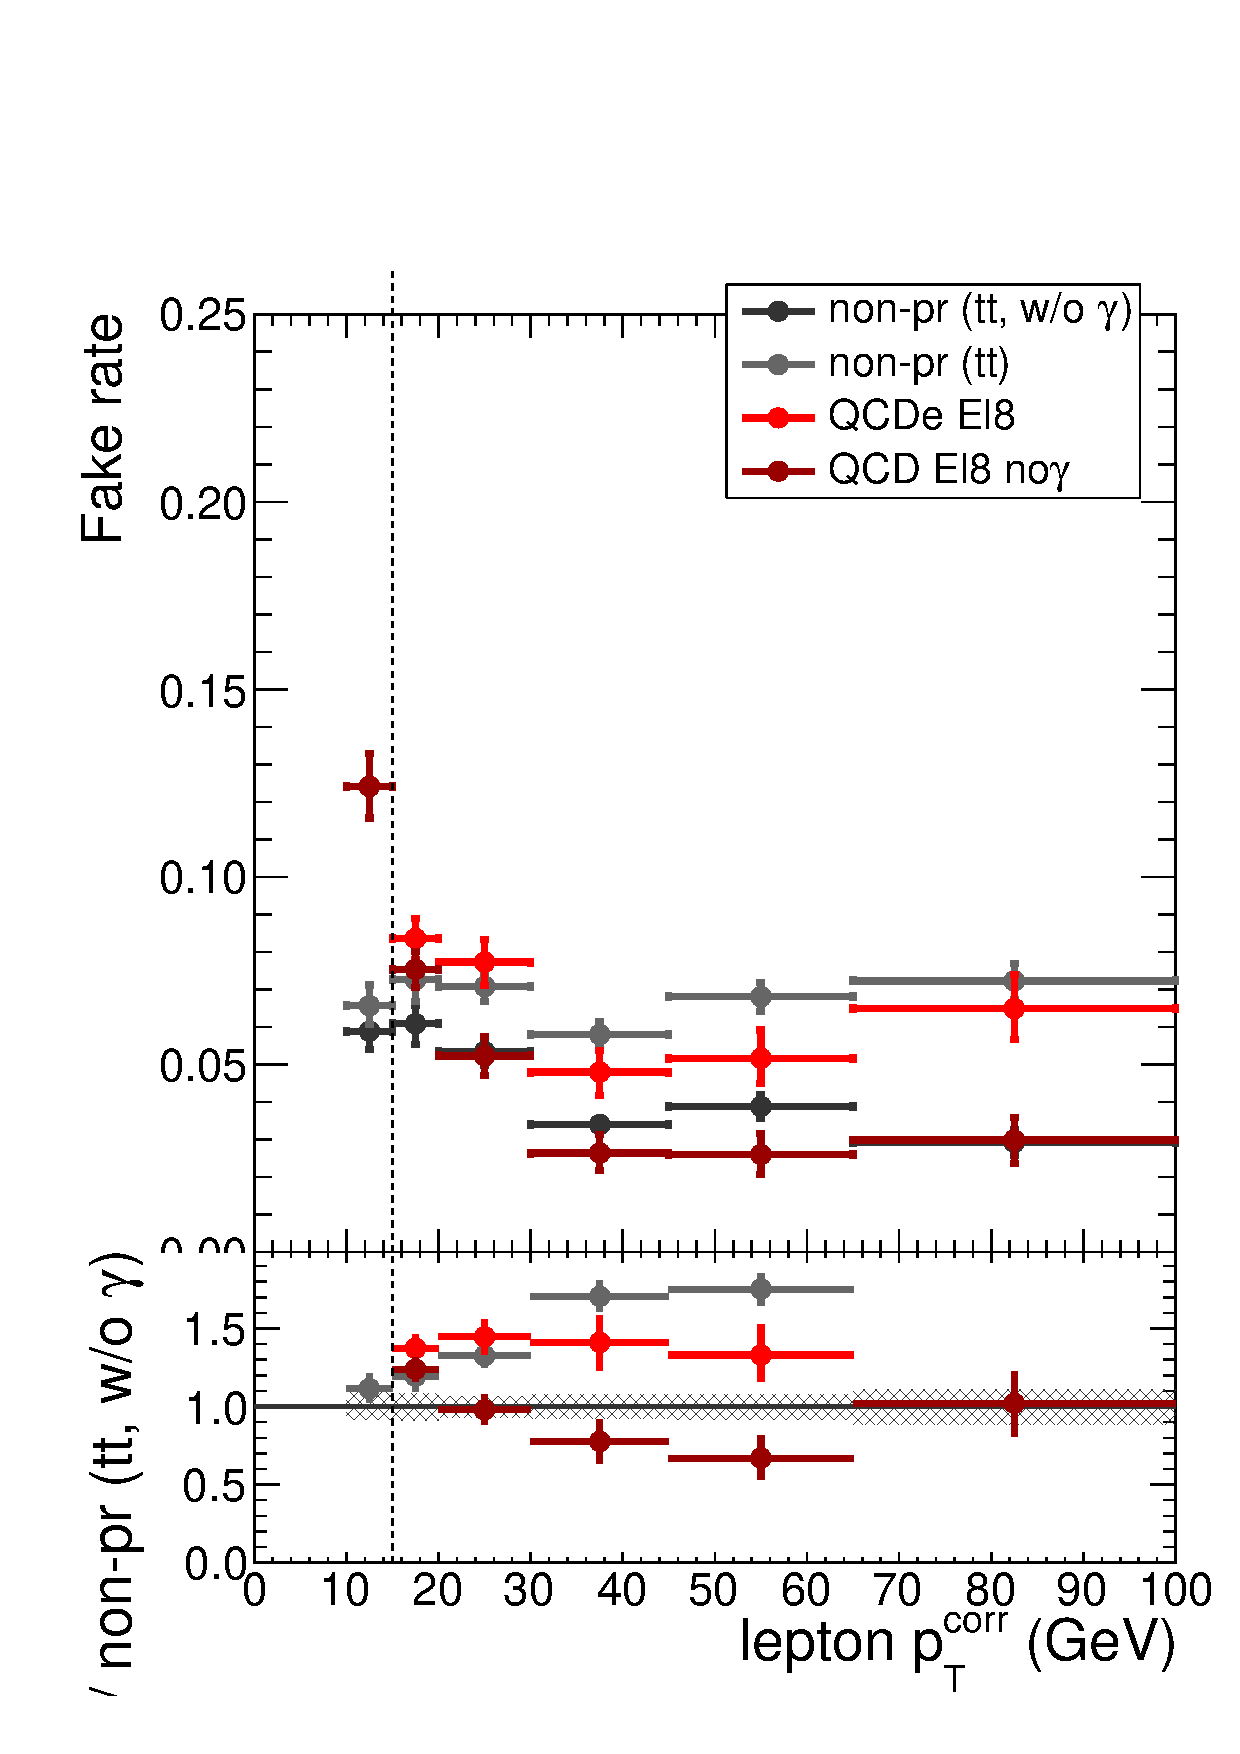
\includegraphics[width=0.35\textwidth]{plots_fakerate/measurement/el_lbin_endcap}
	\caption{Fake rate for background electrons in the barrel (left) and endcaps (right), from simulated $\ttbar$ and QCD events, inclusively or excludning those from the conversions for prompt photons. Electrons in QCD events are required to pass the HLT\_Ele8\_CaloIdM\_TrackIdM\_PFJet30 trigger.}
	\label{fig:frmeas-closure-bnb-el}
\end{figure}

%A comparison of fake rates for QCD events as function of the requirements on the recoiling jet in the QCD selection is illustrated in Fig.~\ref{fig:frmeas-ajpt-ajb}. For both leptons, we observe an excellent stability of the fake rate as function of the recoiling jet \pt, and only a moderate dependency on the b-tagging requirements of the away jet. So, we decide to define the measurement region requiring only $\pt > 30 \GeV$ on the recoling jet, and no b-tagging, to benefit from the largest event sample and reduce the statistical uncertainties in the measurements.
%\begin{figure}[htb]
%        \centering
%\includegraphics[width=0.35\textwidth]{plots_fakerate/measurement/mu_qajb_barrel}
%%\includegraphics[width=0.35\textwidth]{plots_fakerate/measurement/mu_qajb_eta_12_24}
%\includegraphics[width=0.35\textwidth]{plots_fakerate/measurement/el_qajb_barrel}
%%\includegraphics[width=0.35\textwidth]{plots_fakerate/measurement/el_qajb_eta_15_25}
%\includegraphics[width=0.35\textwidth]{plots_fakerate/measurement/mu_qajpt_barrel}
%%\includegraphics[width=0.35\textwidth]{plots_fakerate/measurement/mu_qajpt_eta_12_24}
%\includegraphics[width=0.35\textwidth]{plots_fakerate/measurement/el_qajpt_barrel}
%%\includegraphics[width=0.35\textwidth]{plots_fakerate/measurement/el_qajpt_eta_15_25}
%        \caption{Fake rate for leptons in the barrel in simulated QCD and $\ttbar$ events, as varying the requirement on the recoiling jet. In the top row, different cuts are applied on the b-tagging discriminator of the jet, while in the bottom row different $\pt$ thresholds are applied. Fake rates in the left column are for muons, those in the right column for electrons.}
%        \label{fig:frmeas-ajpt-ajb}
%\end{figure}

\subsubsection{QCD measurement: prompt lepton contamination}
An important challenge in measuring the fake rate in jet events in data is the contamination of prompt leptons, mostly from $\PW$ and $\Z$ production in association with hadronic jets, but also from $\ttbar$. In order to suppres the $\Z$ contamination, events with more than one loose lepton are vetoed, leaving mostly events with one leptons outside the acceptance or from $\Z\to\tau_{\ell}\tau_\mathrm{h}$.
A good discrimination between QCD events and $\PW$ can be achieved from the transverse mass of the lepton and missing energy in the event, $M_\mathrm{T}(\ell,\ETmiss)$. 
The standard procedure is to apply a tight cut $M_\mathrm{T}(\ell,\ETmiss)<15\GeV$ was applied, and the residual contamination was subtracted at numerator and denominator in each \pt bin using simulated $\PW/\Z+\mathrm{jets}$ events. The simulation was normalized to the data from a fit to $M_\mathrm{T}(\ell,\ETmiss)$, in the sample of events at the fake rate numerator (i.e. passing the tight requirements), before the cut at $15\GeV$.

For this analsyis, we implemented two improvements on that procedure. The first improvement is a change in the discriminating variable used: the traditional transverse mass
\[ M_\mathrm{T}(\ell,\ETmiss) = \sqrt{2 {\pt}_\ell \ETmiss (1-\cos\Delta\phi)} \]
is obviously correlated with the lepton \pt, and so also with the lepton fake rate. To avoid this correlation, which can potentially introduce biases in the subtraction procedure, we define a new variable
\[ M_\mathrm{T}^{\mathrm{fix}}(\ell,\ETmiss) := \sqrt{2 {\pt}_{\mathrm{fix}} \ETmiss (1-\cos\Delta\phi)} \]
replacing the lepton \pt with a fixed number ($35\GeV$), and thus relying only on the lepton direction. This variable still has a good discriminating power against $\PW+\mathrm{jets}$ but is much less correlated with the lepton $\pt$ and so with the fake rate.

The second improvement is the introduction of two alternative ways to implement the subtraction of the prompt contamination. The first alternative procedure is the one used in the run 1 analysis, and documented in detail in Section~7.4.2 of AN-13-159, except that we update it to use $M_\mathrm{T}^{\mathrm{fix}}(\ell,\ETmiss)$ instead of $\ETmiss$. The procedure relies on two measurement of the fake rate in data, one for small $M_\mathrm{T}^{\mathrm{fix}}$ values and one for 
large and large $M_\mathrm{T}^{\mathrm{fix}}$ values. Assuming the fake rate to be independent from $M_\mathrm{T}^{\mathrm{fix}}$, and taking from the simulation the ratio of $\mathrm{V}+\mathrm{jets}$ events expected in the two regions, it is possible to unfold the fake rate for QCD events from the two measurements:
\[ f_\mathrm{QCD}  = \frac{f_\mathrm{S} - r^\mathrm{SL}_\mathrm{V+j} f_\mathrm{L}}{1 - r^\mathrm{SL}_\mathrm{V+j}} \qquad 
    \text{where}\quad r^\mathrm{SL}_\mathrm{V+j} = \left(\frac{N^\mathrm{S}_\mathrm{V+j}}{N^\mathrm{S}_\mathrm{V+j}}\right) / \left(\frac{N^\mathrm{S}_\mathrm{data}}{N^\mathrm{L}_\mathrm{data}}\right)\ , \]
where $f_i$ are the fake rates measured in data for small (S) and large (L) values of $M_\mathrm{T}^{\mathrm{fix}}$, $N^i_\mathrm{V+j}$ are the expected event yields from $\mathrm{V}+\mathrm{jets}$ and $N^i_\mathrm{data}$ are the observed events in data in the two regions at the denominator of the fake rate. This procedure can be performed separately in each bin of \pt, $|\eta|$. 

In this version of the analysis, a small refinement of the procedure is done to account for the observed residual dependency of the fake rate on $M_\mathrm{T}^{\mathrm{fix}}$ from MC: the formula is modified to 
    \[ f_\mathrm{QCD}  = \frac{f_\mathrm{S} - \mu\,r^\mathrm{SL}_\mathrm{V+j}\,f_\mathrm{L}}{1 - \mu\,\gamma\,r^\mathrm{SL}_\mathrm{V+j} + \frac{N^\mathrm{S}_\mathrm{V+j}}{N^\mathrm{S}_\mathrm{V+j}+N^\mathrm{S}_\mathrm{QCD}} (\mu \gamma - 1)} \]
where $\mu = \epsilon^\mathrm{V+j}_\mathrm{S}/\epsilon^\mathrm{V+j}_\mathrm{L}$ and $\gamma = \epsilon^\mathrm{QCD}_\mathrm{L}/\epsilon^\mathrm{QCD}_\mathrm{S}$, and $f_\mathrm{QCD}$ is defined as $\epsilon^\mathrm{QCD}_\mathrm{S}$ since the bulk of the QCD events have low $\ETmiss$. In addition to the statistical uncertainties from data and MC, we assign a systematical uncertainty of $100\%$ on the corrections (i.e on $\gamma-1$, $\mu-1$ and ${N^\mathrm{S}_\mathrm{V+j}}/({N^\mathrm{S}_\mathrm{V+j}+N^\mathrm{S}_\mathrm{QCD}})$) since they are derived from MC and not data.

A second alternative procedure relies on a simultaneous fit of the $M_\mathrm{T}^{\mathrm{fix}}$ distribution for passing and failing probes, in a very similar way to the method used in the tag and probe method at the \Z peak by fitting the invariant mass of the dilepton pair to extract efficiencies for the signal even in the presence of background . In our case, fit is done using templates from simulation for the QCD and $\mathrm{V}+\mathrm{jets}$ contributions. In addition to bin-by-bin statistical uncertainties on the templates, we include systematic shape uncertainties on the templates: we allow both a linear deformation of the template and a stretching of the template, as illustrated in Fig.~\ref{fig:frmeas-shapesyst}. The shape systematics are assumed to be uncorrelated between QCD and $\mathrm{V}+\mathrm{jets}$, but totally correlated between passing and failing probes; the size of the deformation has been chosen to approximately cover the data to simulation differences observed across the various bins. The final uncertainty on the fake rate is obtained by profiling the likelihood of the simultaneous fit, and thus includes both the statistical and the systematical uncertainties.
\begin{figure}[htb]
	\centering 
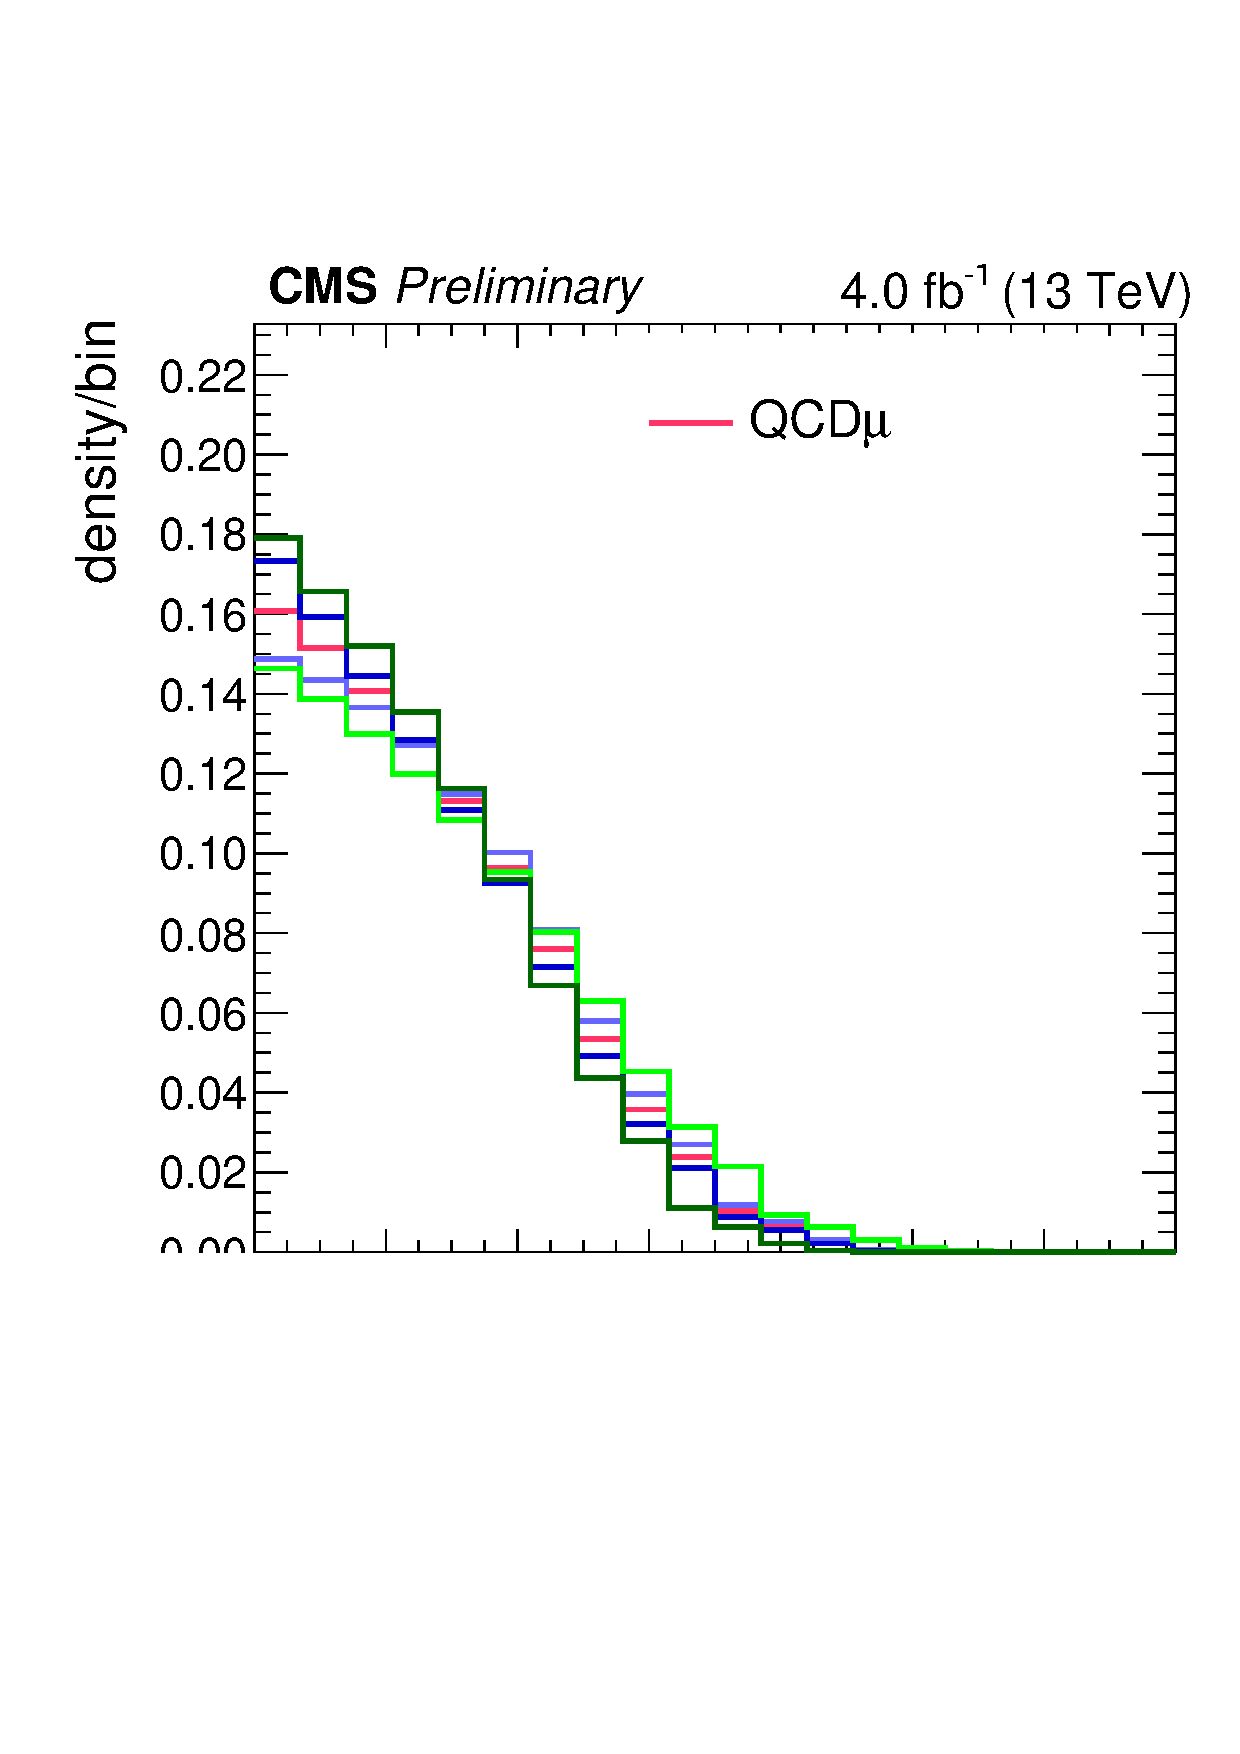
\includegraphics[width=0.35\textwidth]{plots_fakerate/measurement/mu_fitSimND_bin_20_30_pass_sigSyst}
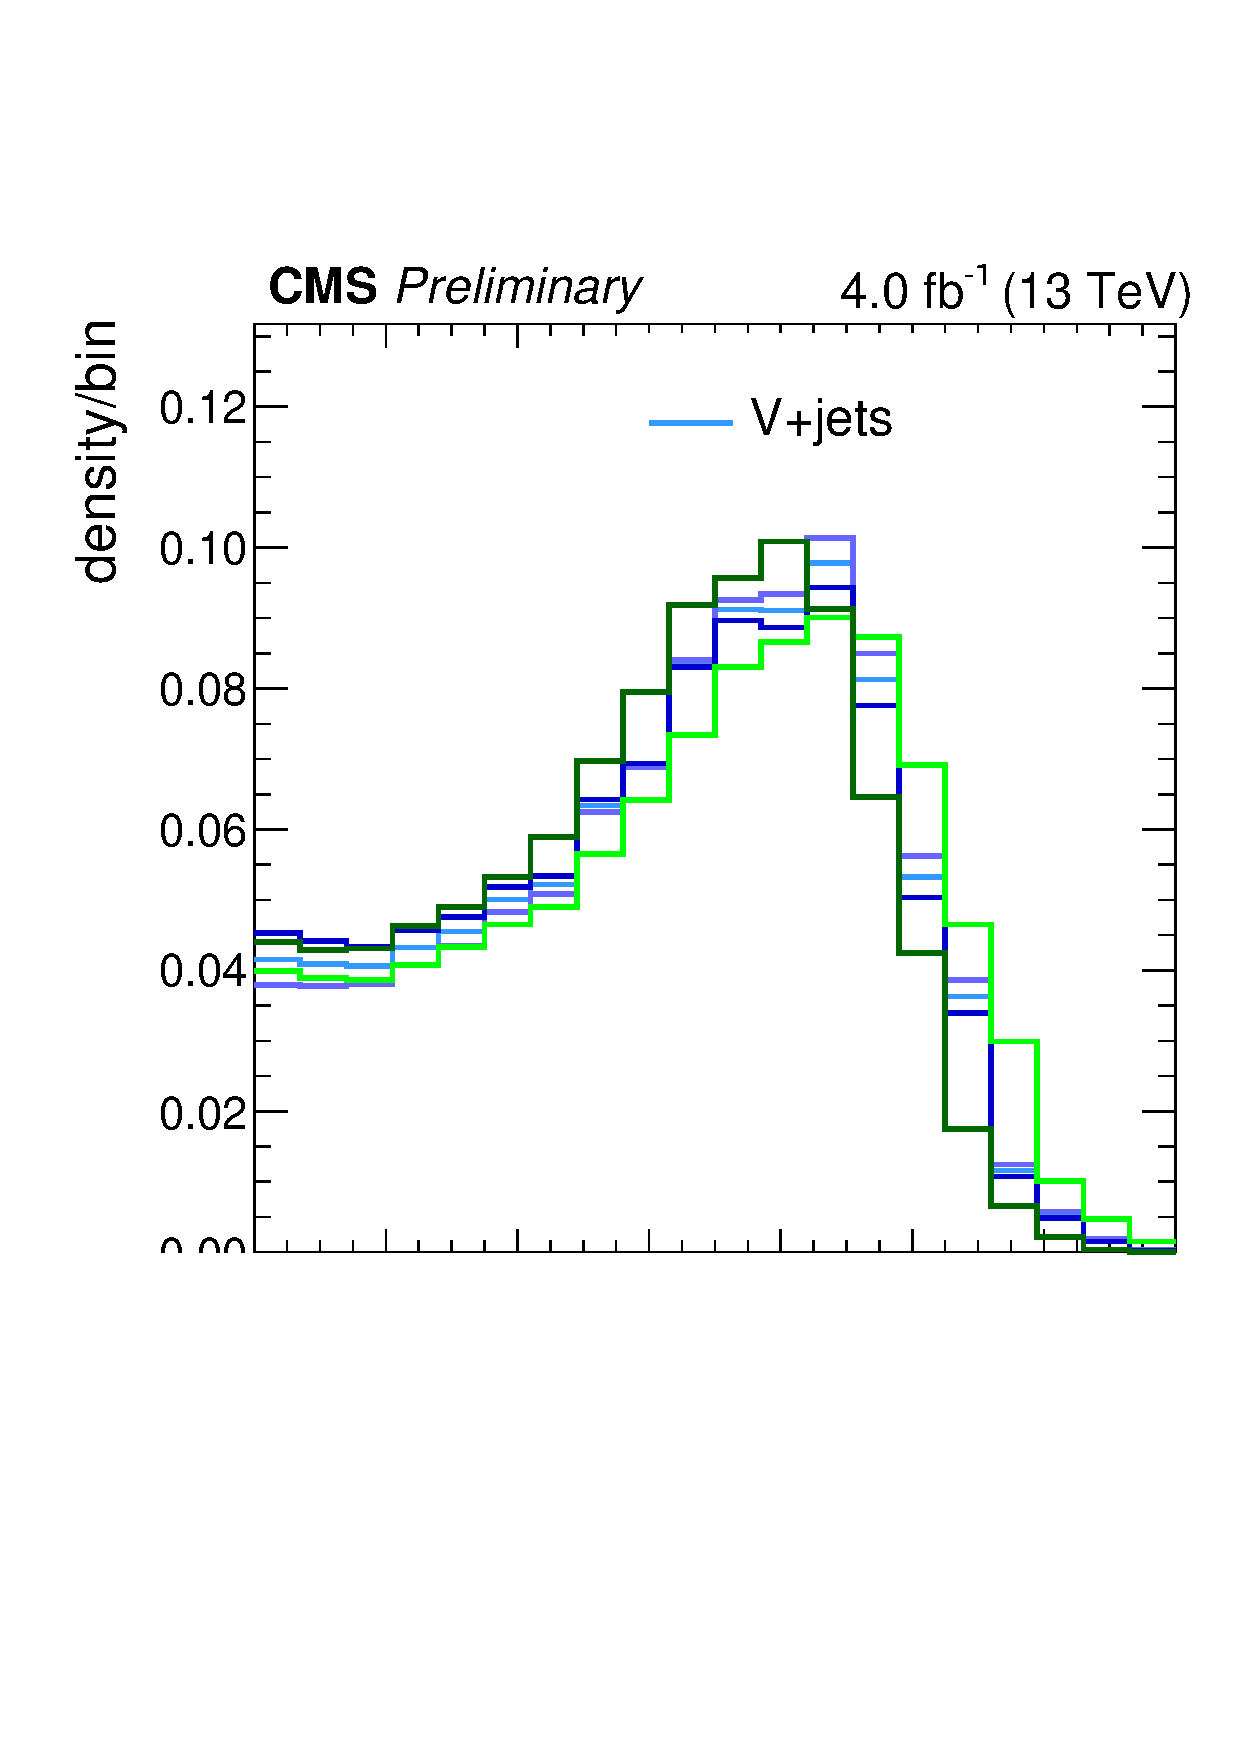
\includegraphics[width=0.35\textwidth]{plots_fakerate/measurement/mu_fitSimND_bin_20_30_pass_bkgSyst}
	\caption{Shape uncertainties on the $M_\mathrm{T}^{\mathrm{fix}}$ templates for muons in the barrel, in the bin of corrected $\pt$ $20$--$30\GeV$, for QCD events (left) and $\mathrm{V}+\mathrm{jets}$ events (right)}
	\label{fig:frmeas-shapesyst}
\end{figure}

Results of the measurement with all three subtraction methods are shown in Fig.~\ref{fig:frmeas-qcd-data-methods}. For the cut and subtraction method, the error bars include a systematical uncertainty of $5\%$ on the subtraction, which dominates over the statistical uncertainties at larger $\pt$. Within uncertainties, the three methods agree among themselves and also with the fake rate in MC. Since we do expect at least some correlation in the uncertainties of the three measurements, we opt for a conservative combination of the three by taking as uncertainty band the envelope of the three uncertainty bands and as central value the midpoint of the band.
\begin{figure}[htb]
        \centering
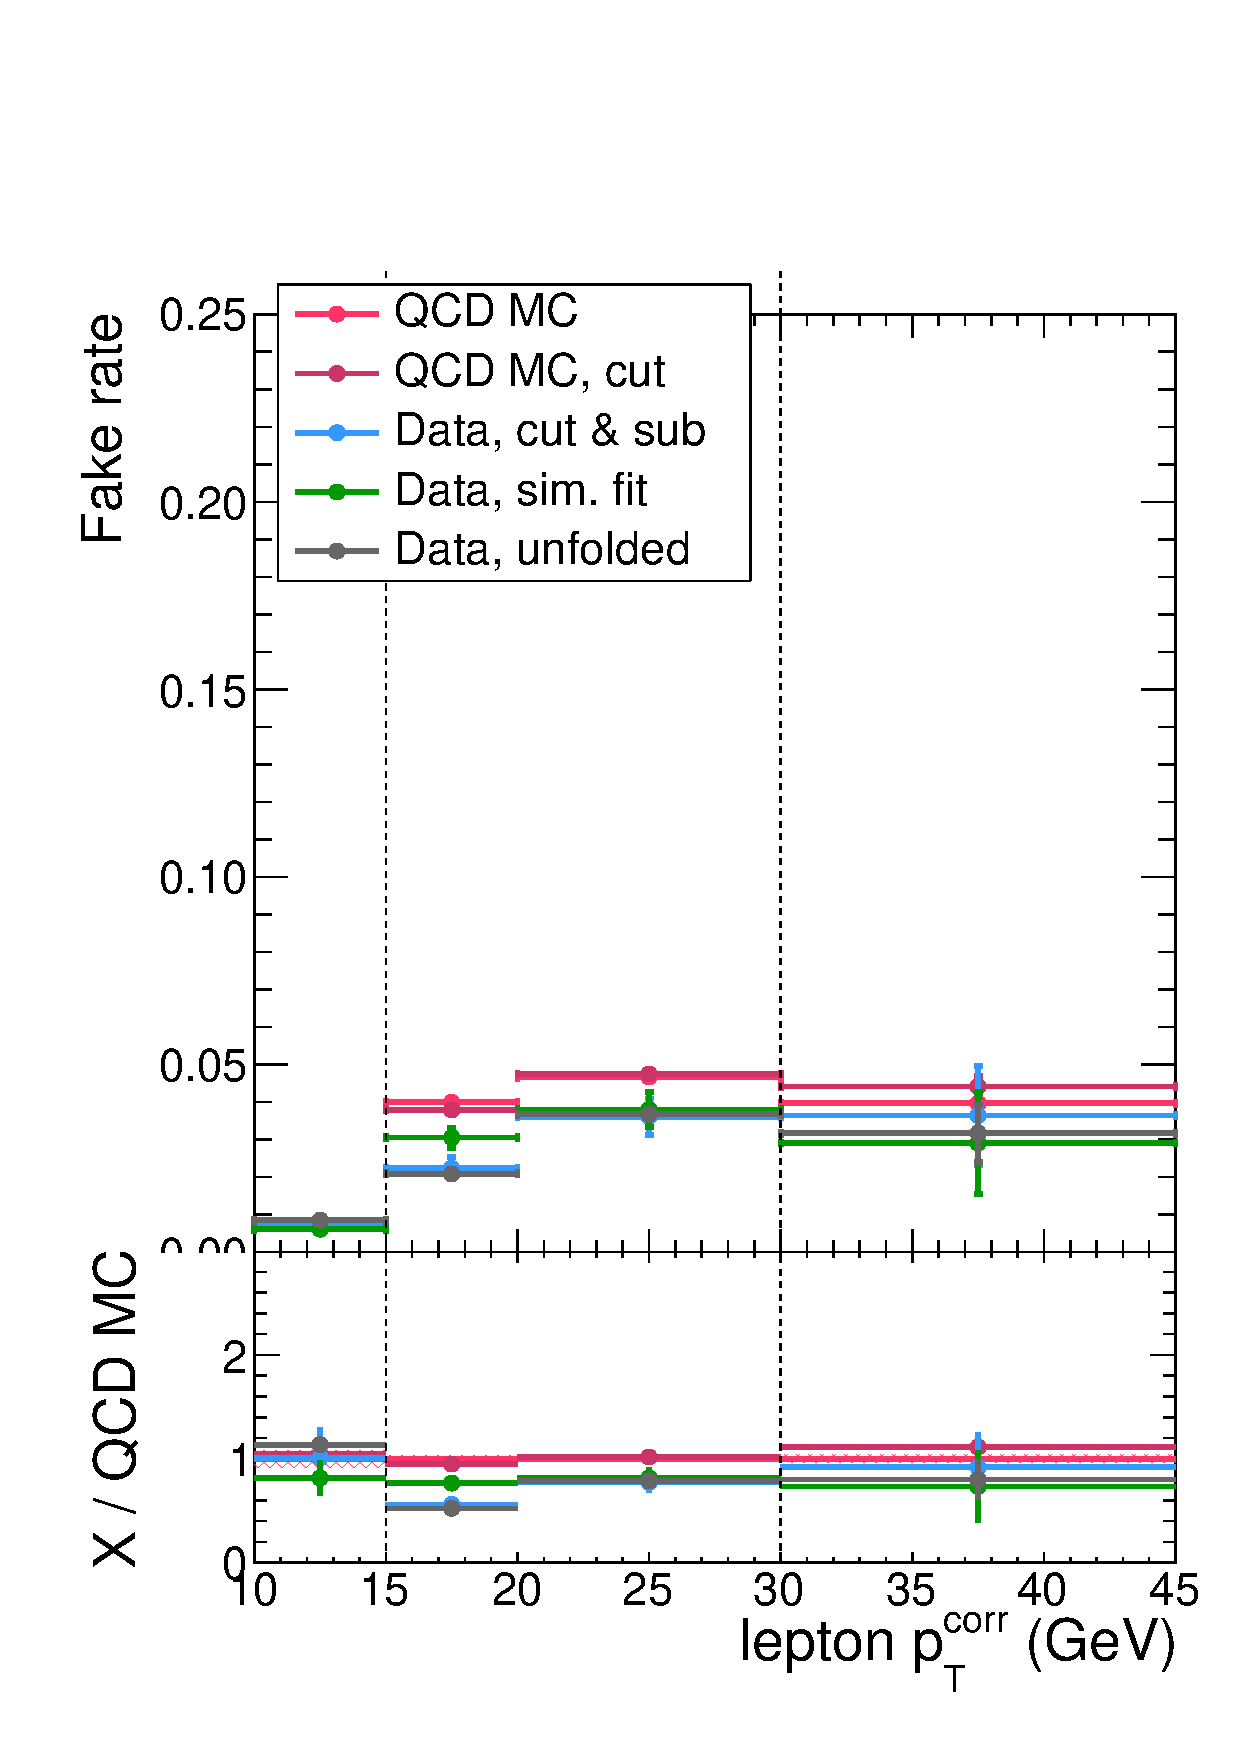
\includegraphics[width=0.32\textwidth]{plots_fakerate/measurement/fr_MuX_CombLow_eta_00_12_comp}
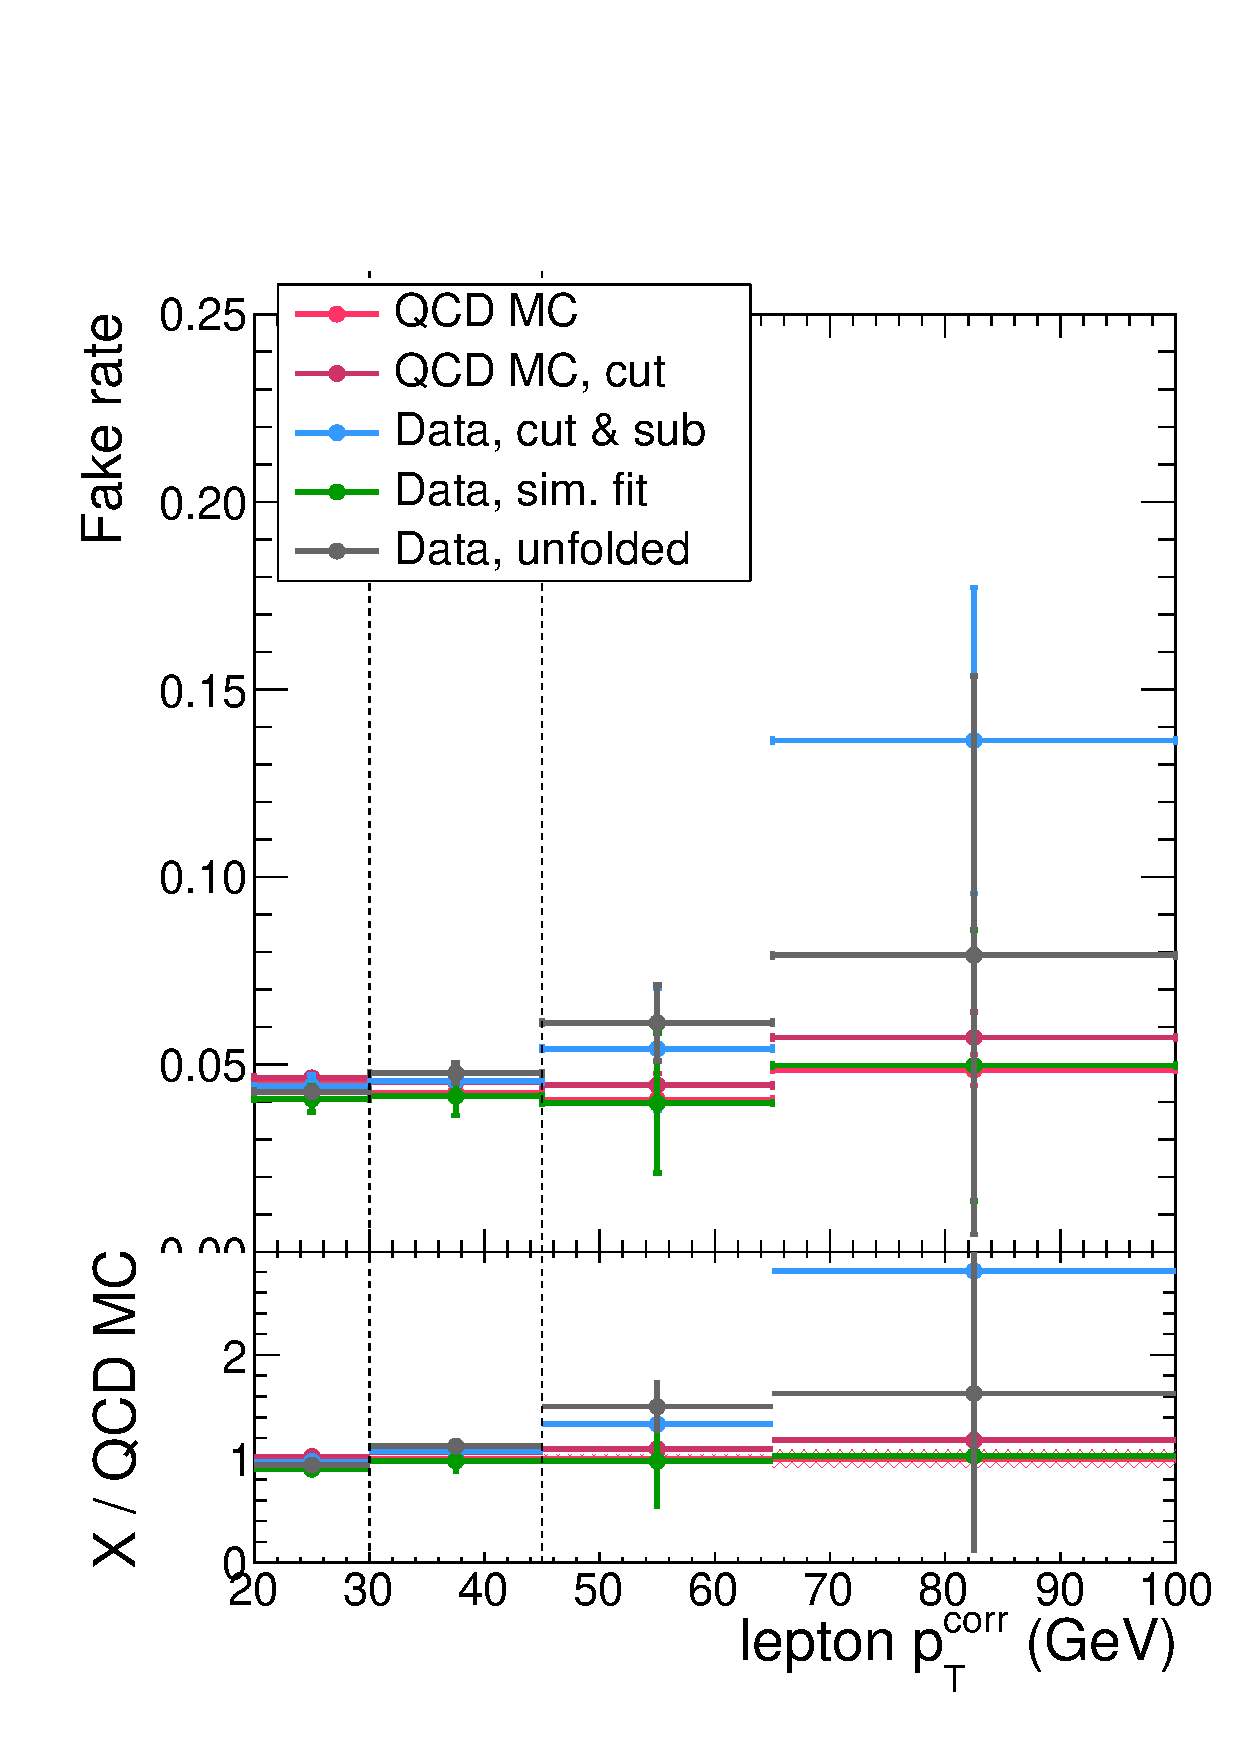
\includegraphics[width=0.32\textwidth]{plots_fakerate/measurement/fr_MuX_CombHigh_eta_00_12_comp}
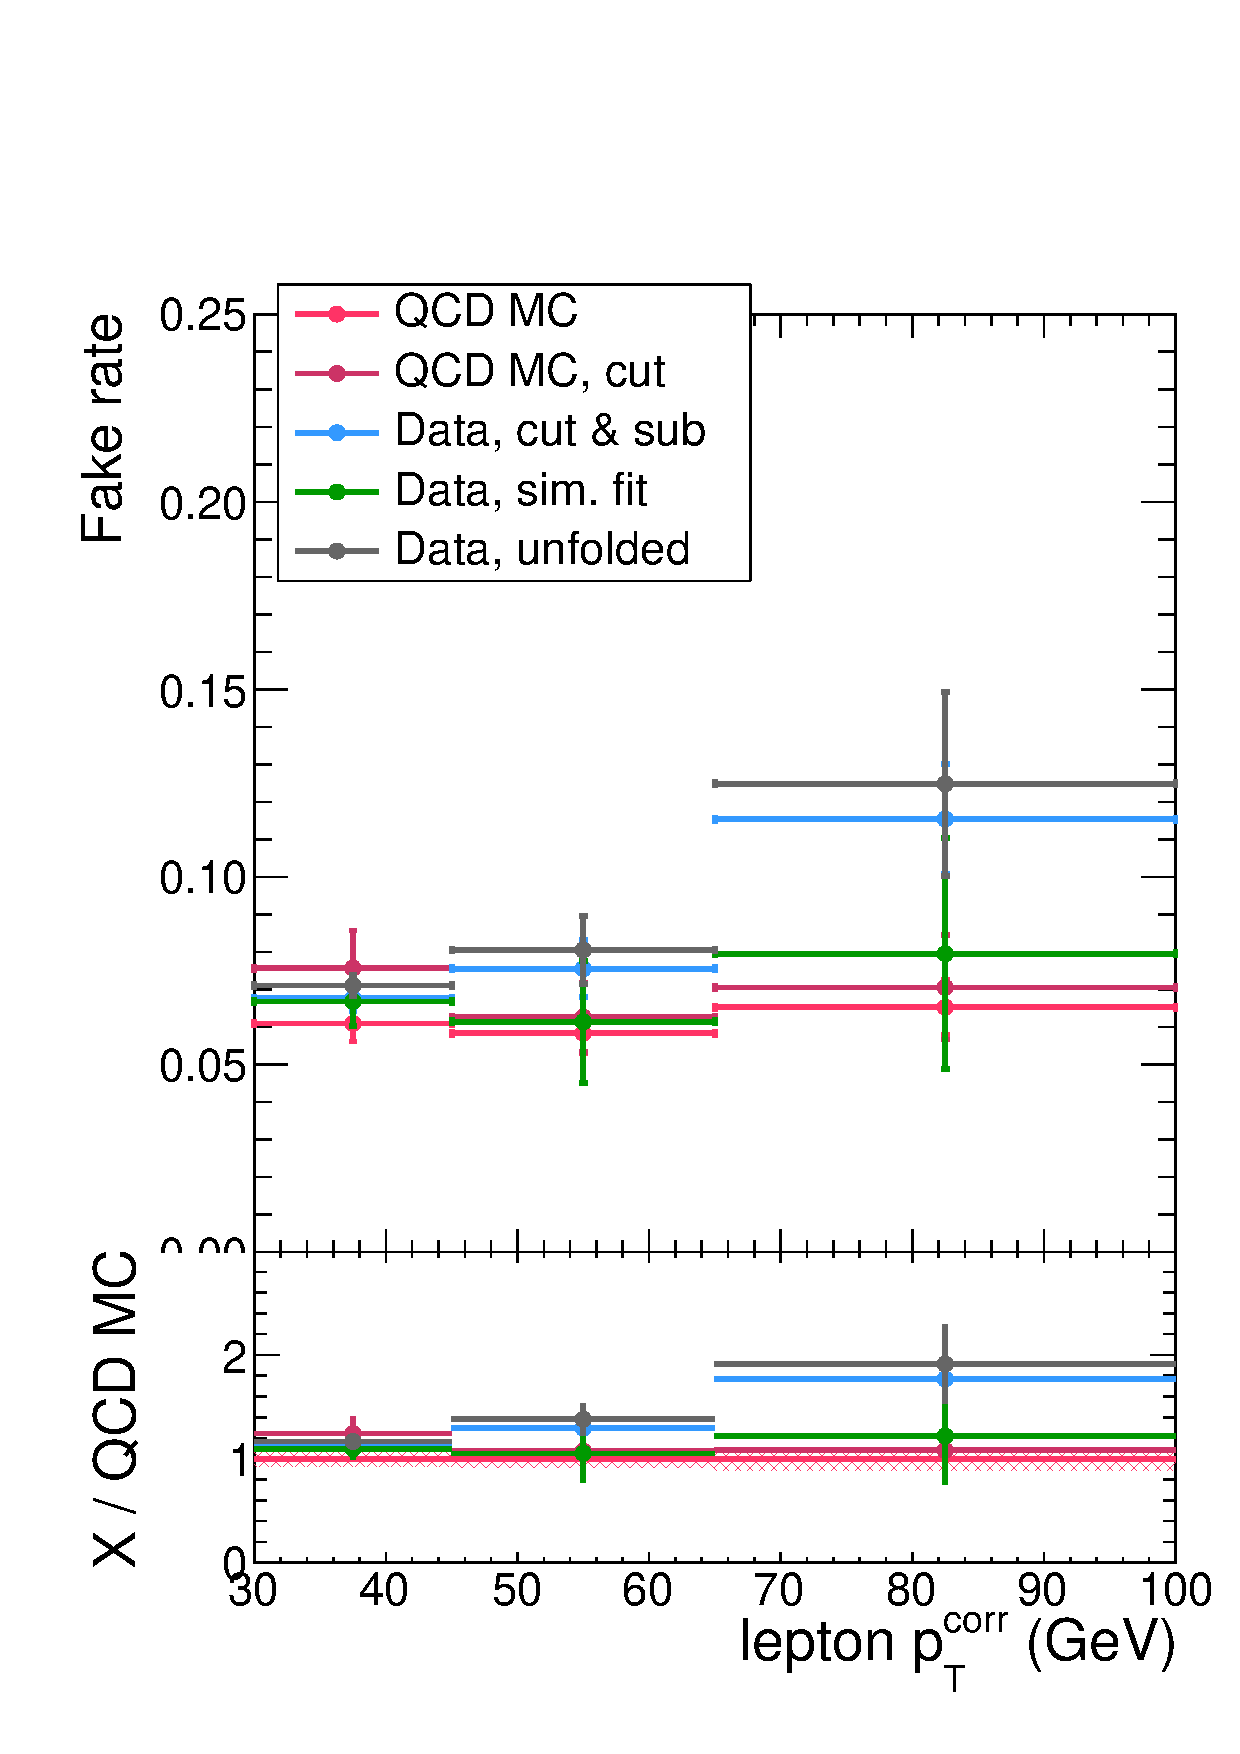
\includegraphics[width=0.32\textwidth]{plots_fakerate/measurement/fr_Ele17_eta_00_15_comp}  \\
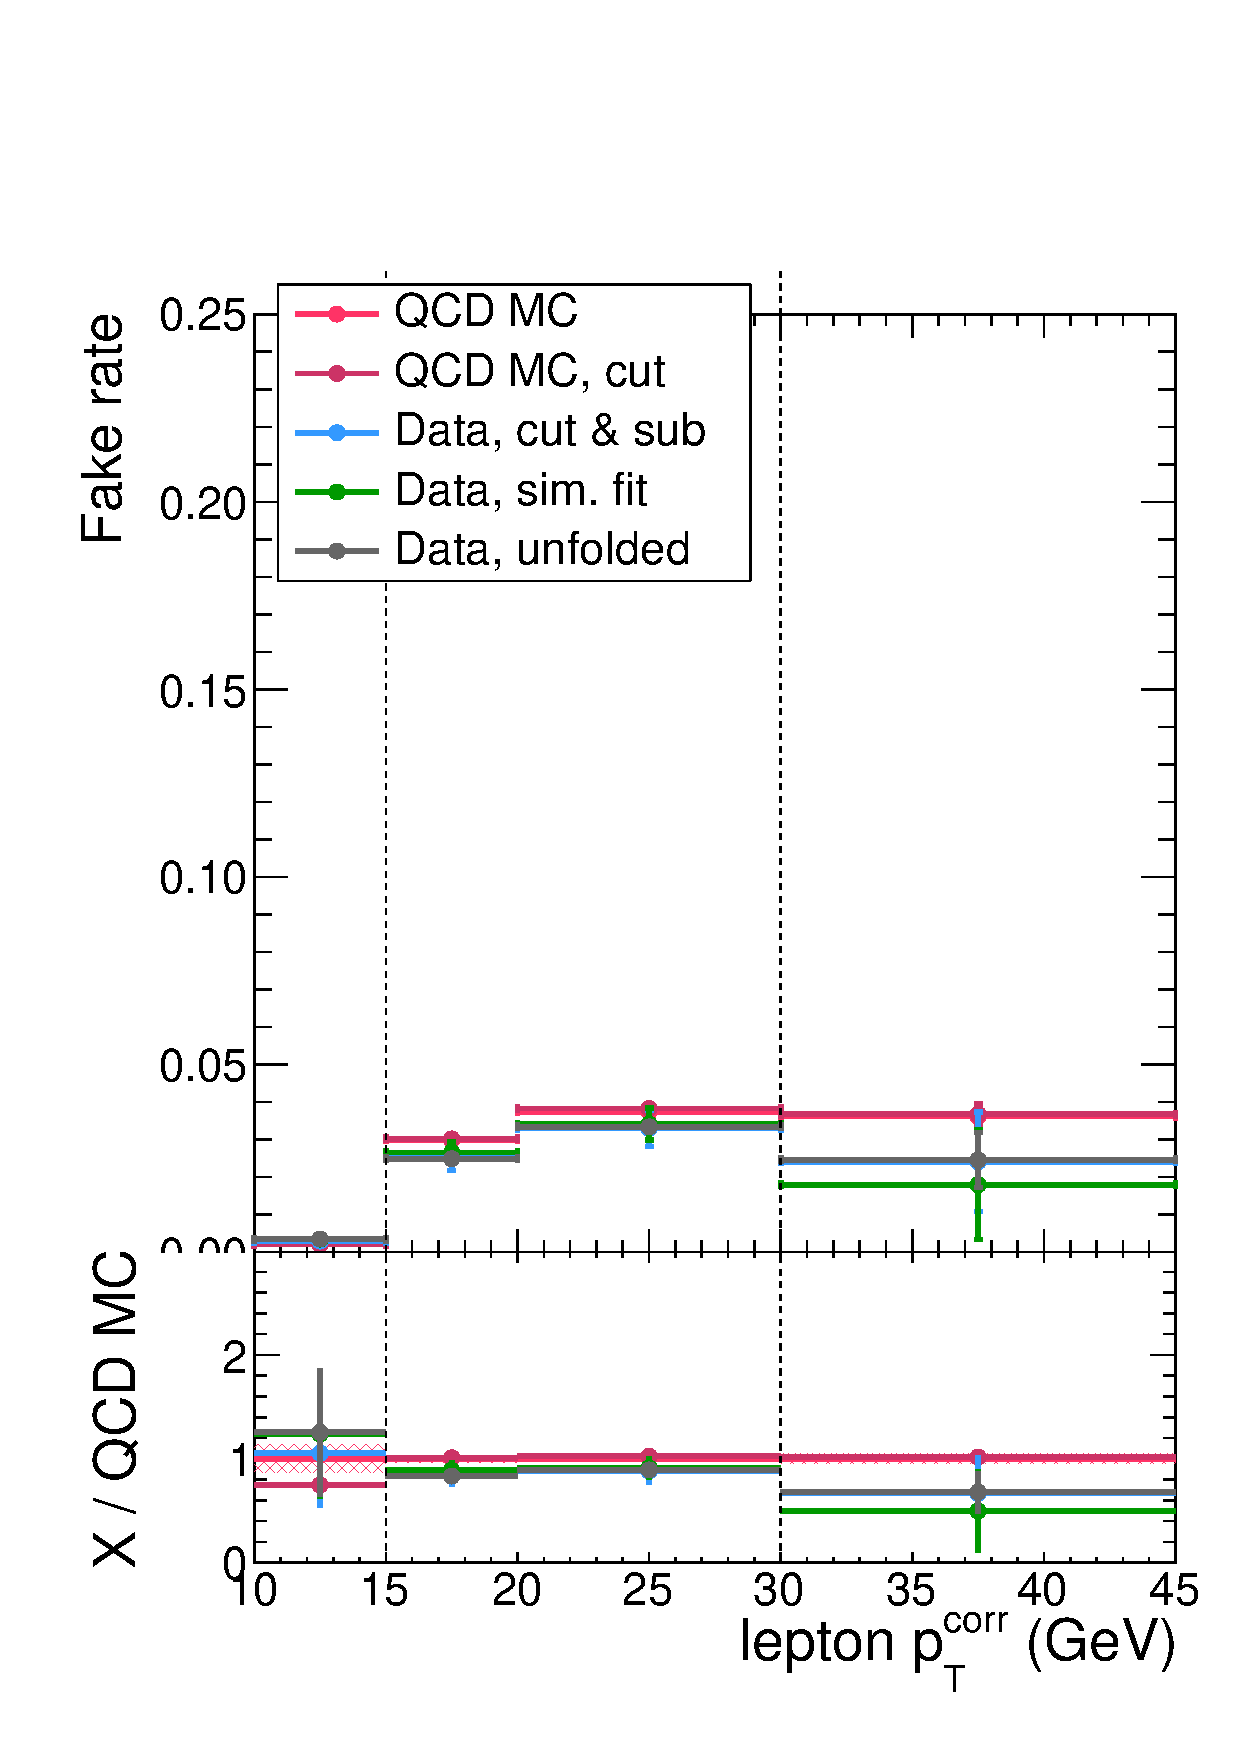
\includegraphics[width=0.32\textwidth]{plots_fakerate/measurement/fr_MuX_CombLow_eta_12_24_comp} 
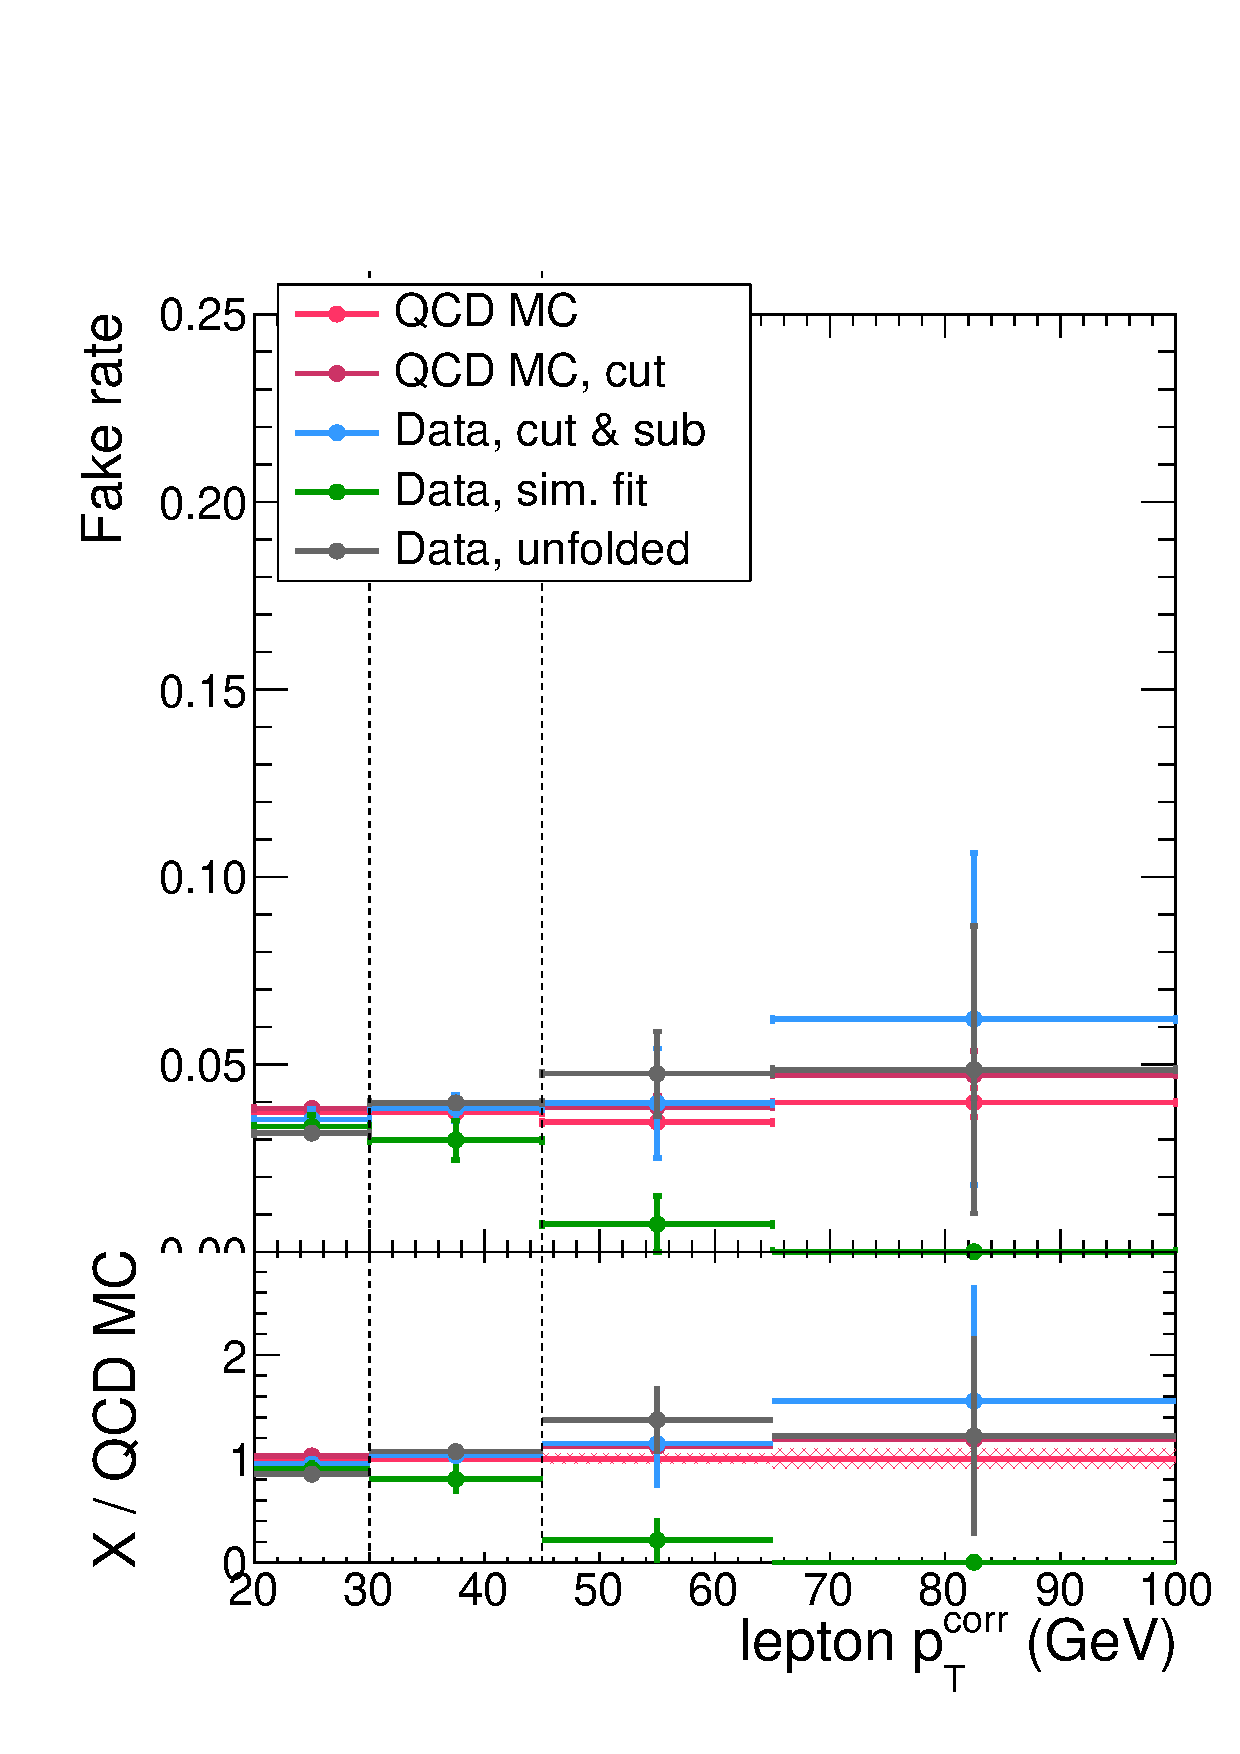
\includegraphics[width=0.32\textwidth]{plots_fakerate/measurement/fr_MuX_CombHigh_eta_12_24_comp}
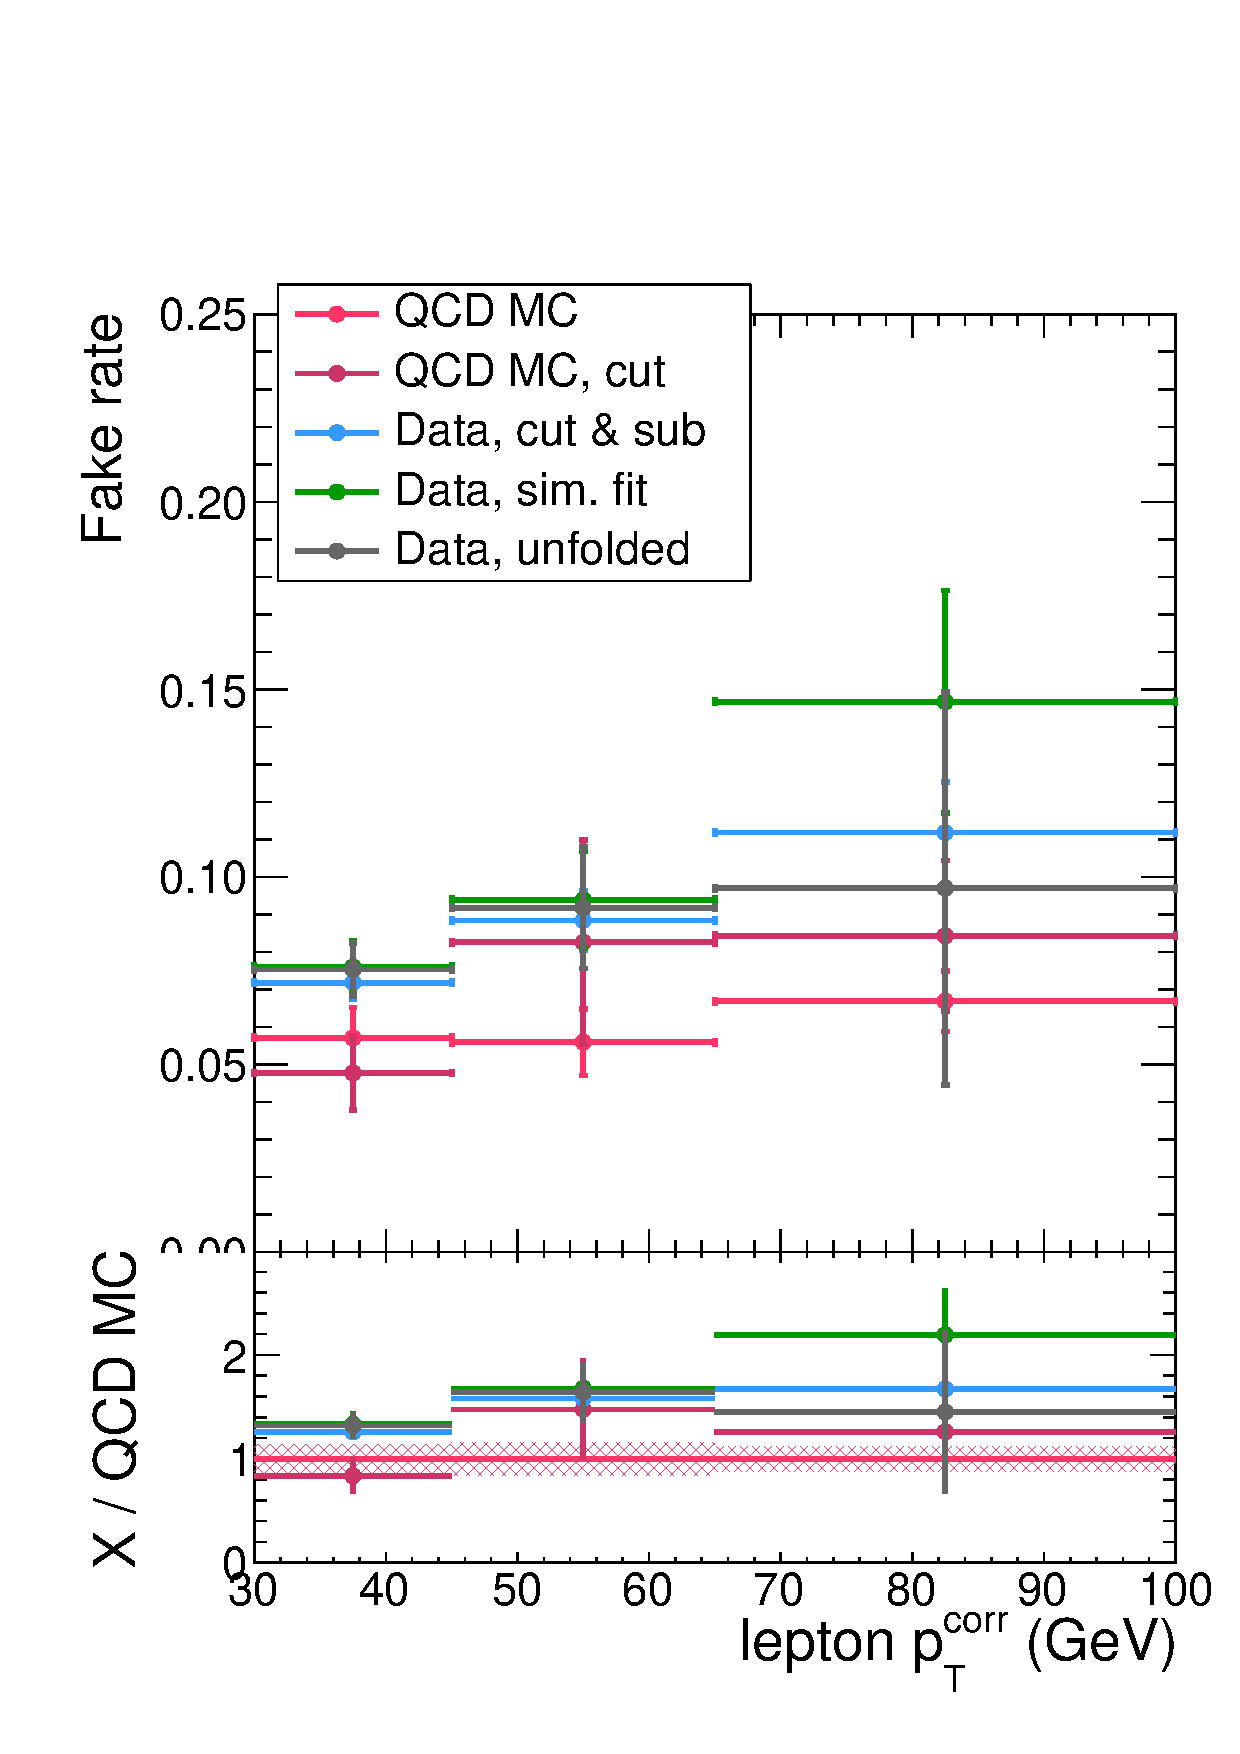
\includegraphics[width=0.32\textwidth]{plots_fakerate/measurement/fr_Ele17_eta_15_25_comp}
        \caption{Fake rate measurement in data, for different subtraction methods, and compared with the predictions from simulation for non-prompt leptons from QCD MC. The top row is for the barrel, the bottom for the endcaps. The left column is for low $\pt$ muons, the middle one for high $\pt$ muons, and the right one for high $\pt$ electrons.}
        \label{fig:frmeas-qcd-data-methods}
\end{figure}

\subsubsection{Results}
The final fake rates for electrons and muons are shown in Fig.~\ref{fig:frmeas-comb-data}. Overall, a good agreement between data and predictions from simulations is observed. Uncertainties are larger for high \pt leptons driven by the uncertainties on the subtraction of the prompt lepton contamination. For electrons, we estimate the fake rate for electrons not from prompt photon conversions by rescaling the measured fake rate in data by the ratio of the fake rates from QCD MC excluding and including electrons from conversions (from Fig.~\ref{fig:frmeas-closure-bnb-el}).
 \begin{figure}[htb]
          \centering
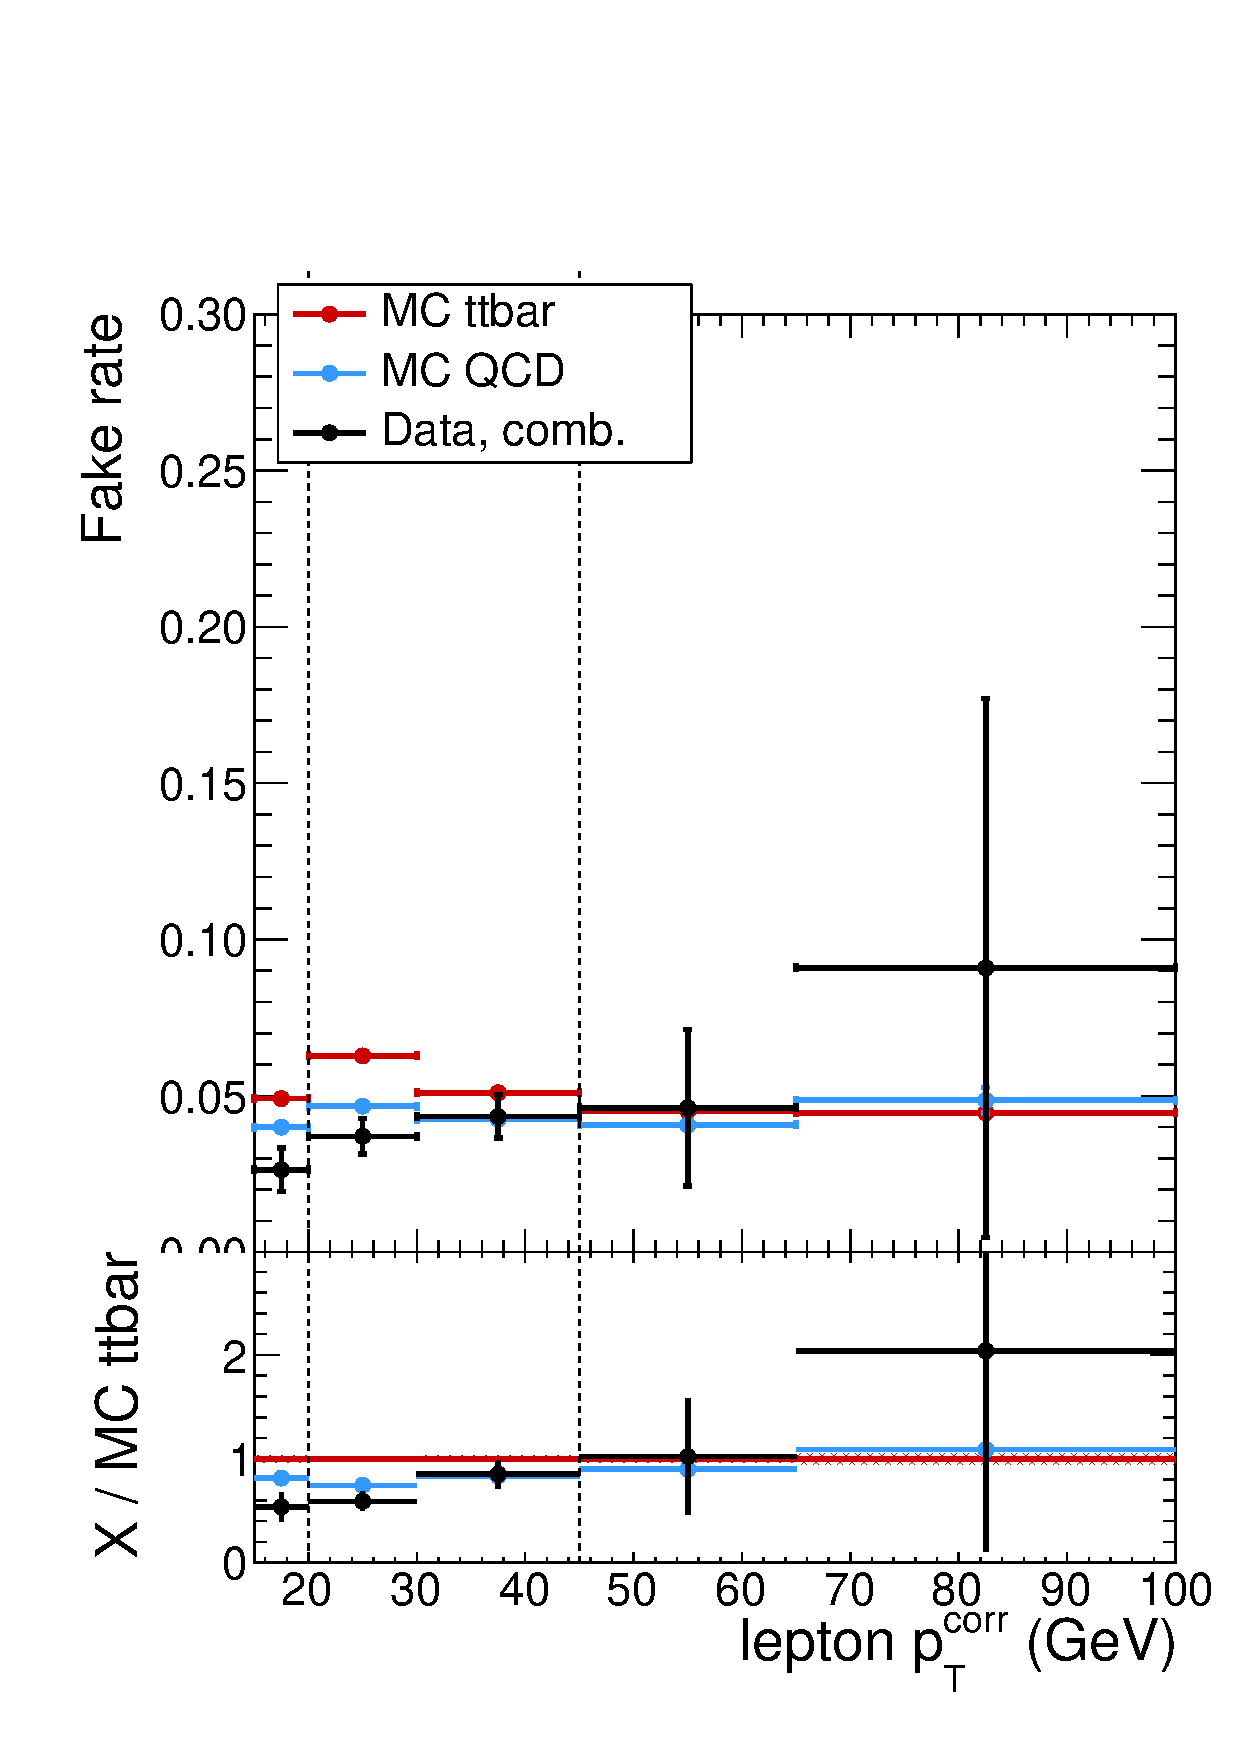
\includegraphics[width=0.35\textwidth]{plots_fakerate/measurement/fr_mu_barrel} 
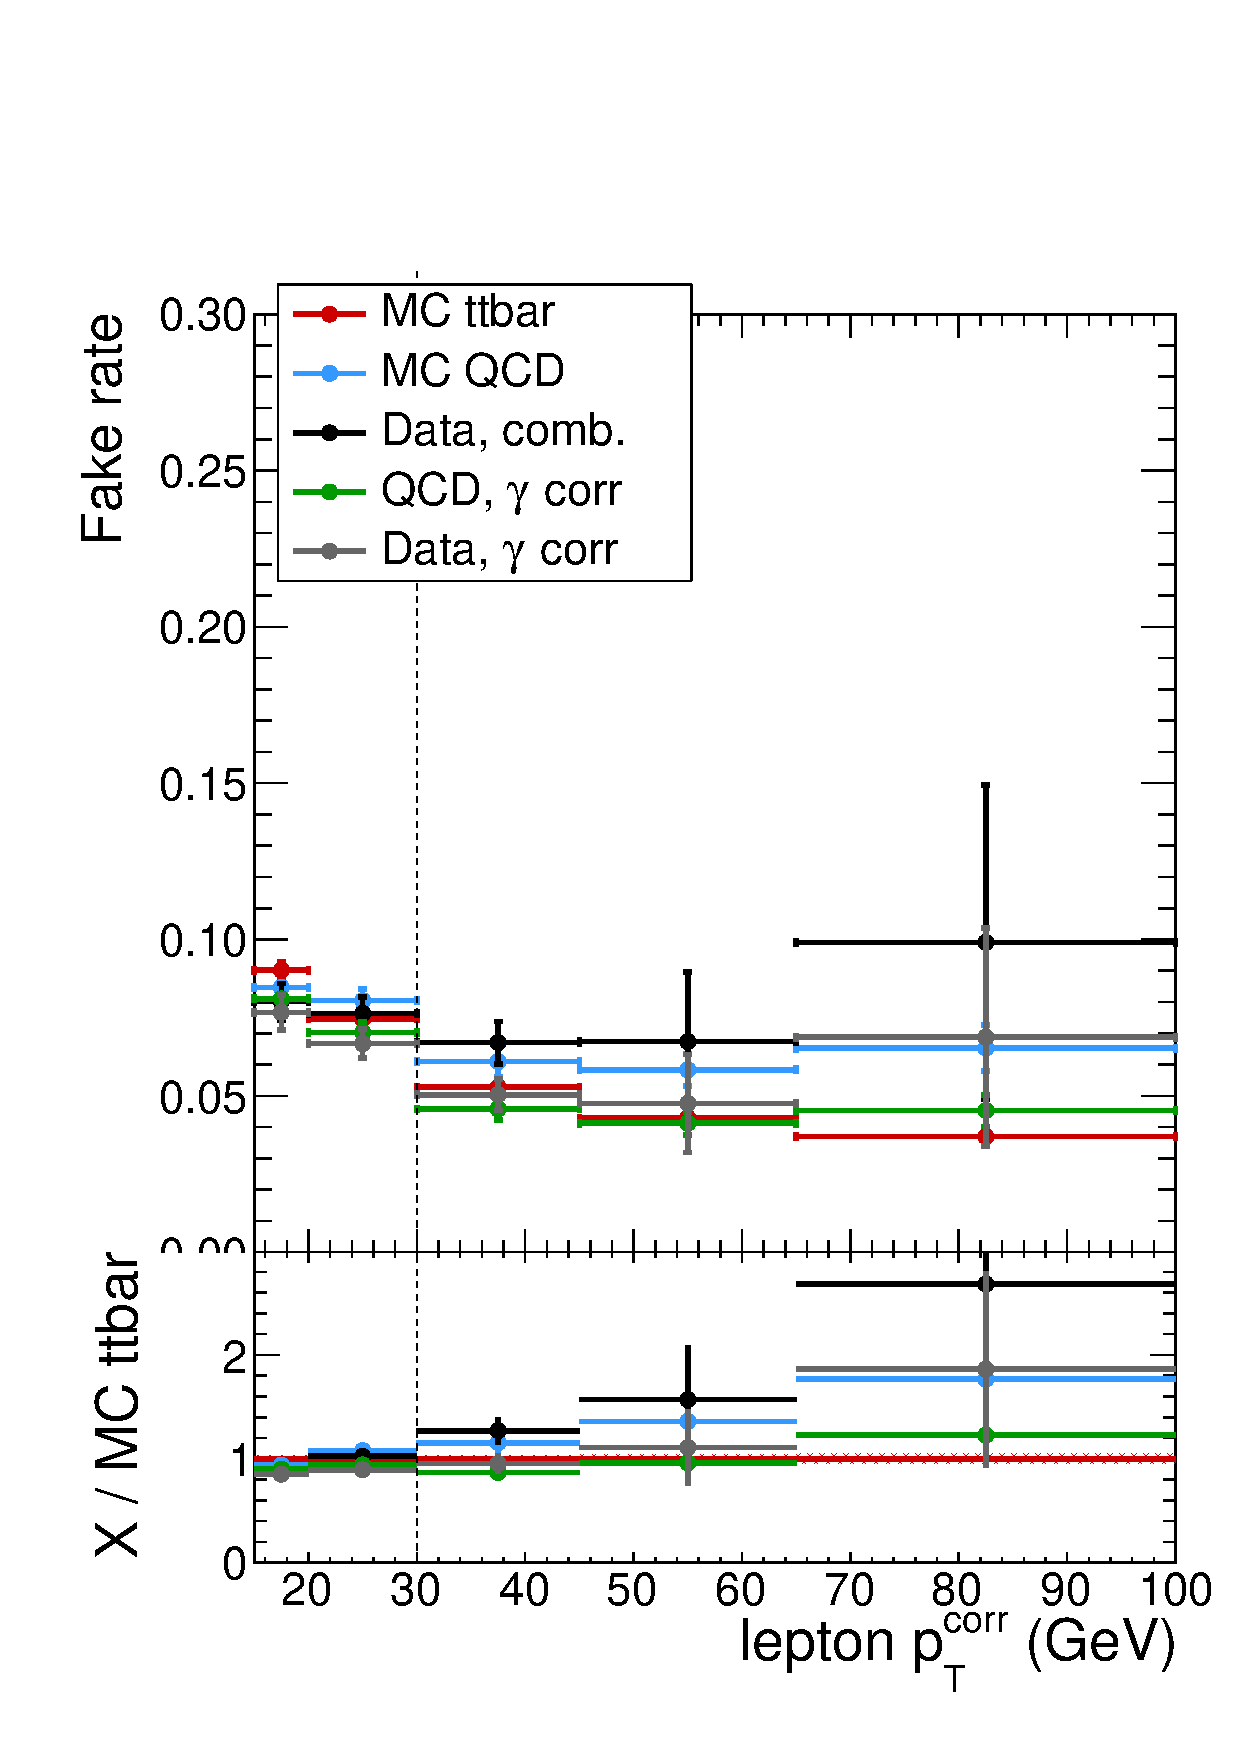
\includegraphics[width=0.35\textwidth]{plots_fakerate/measurement/fr_el_barrel} \\
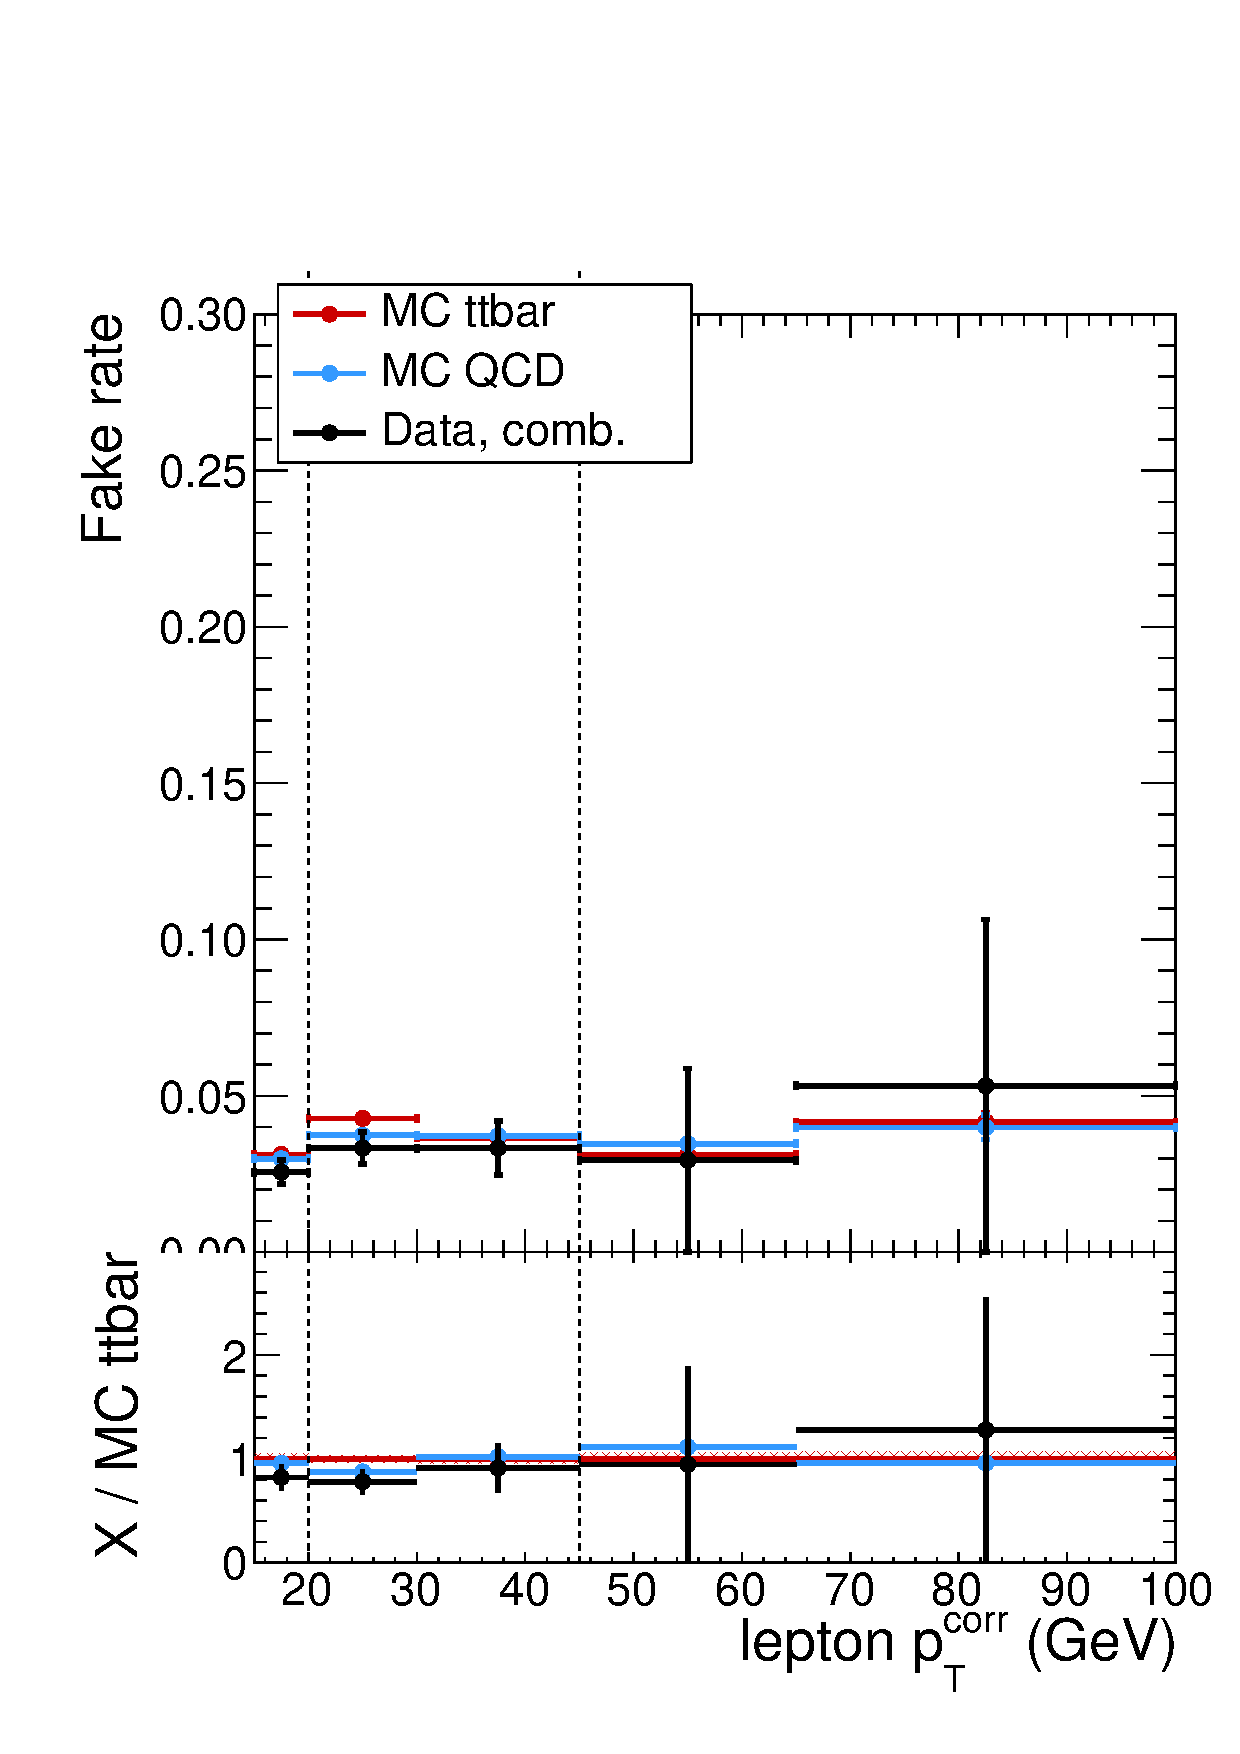
\includegraphics[width=0.35\textwidth]{plots_fakerate/measurement/fr_mu_endcap}
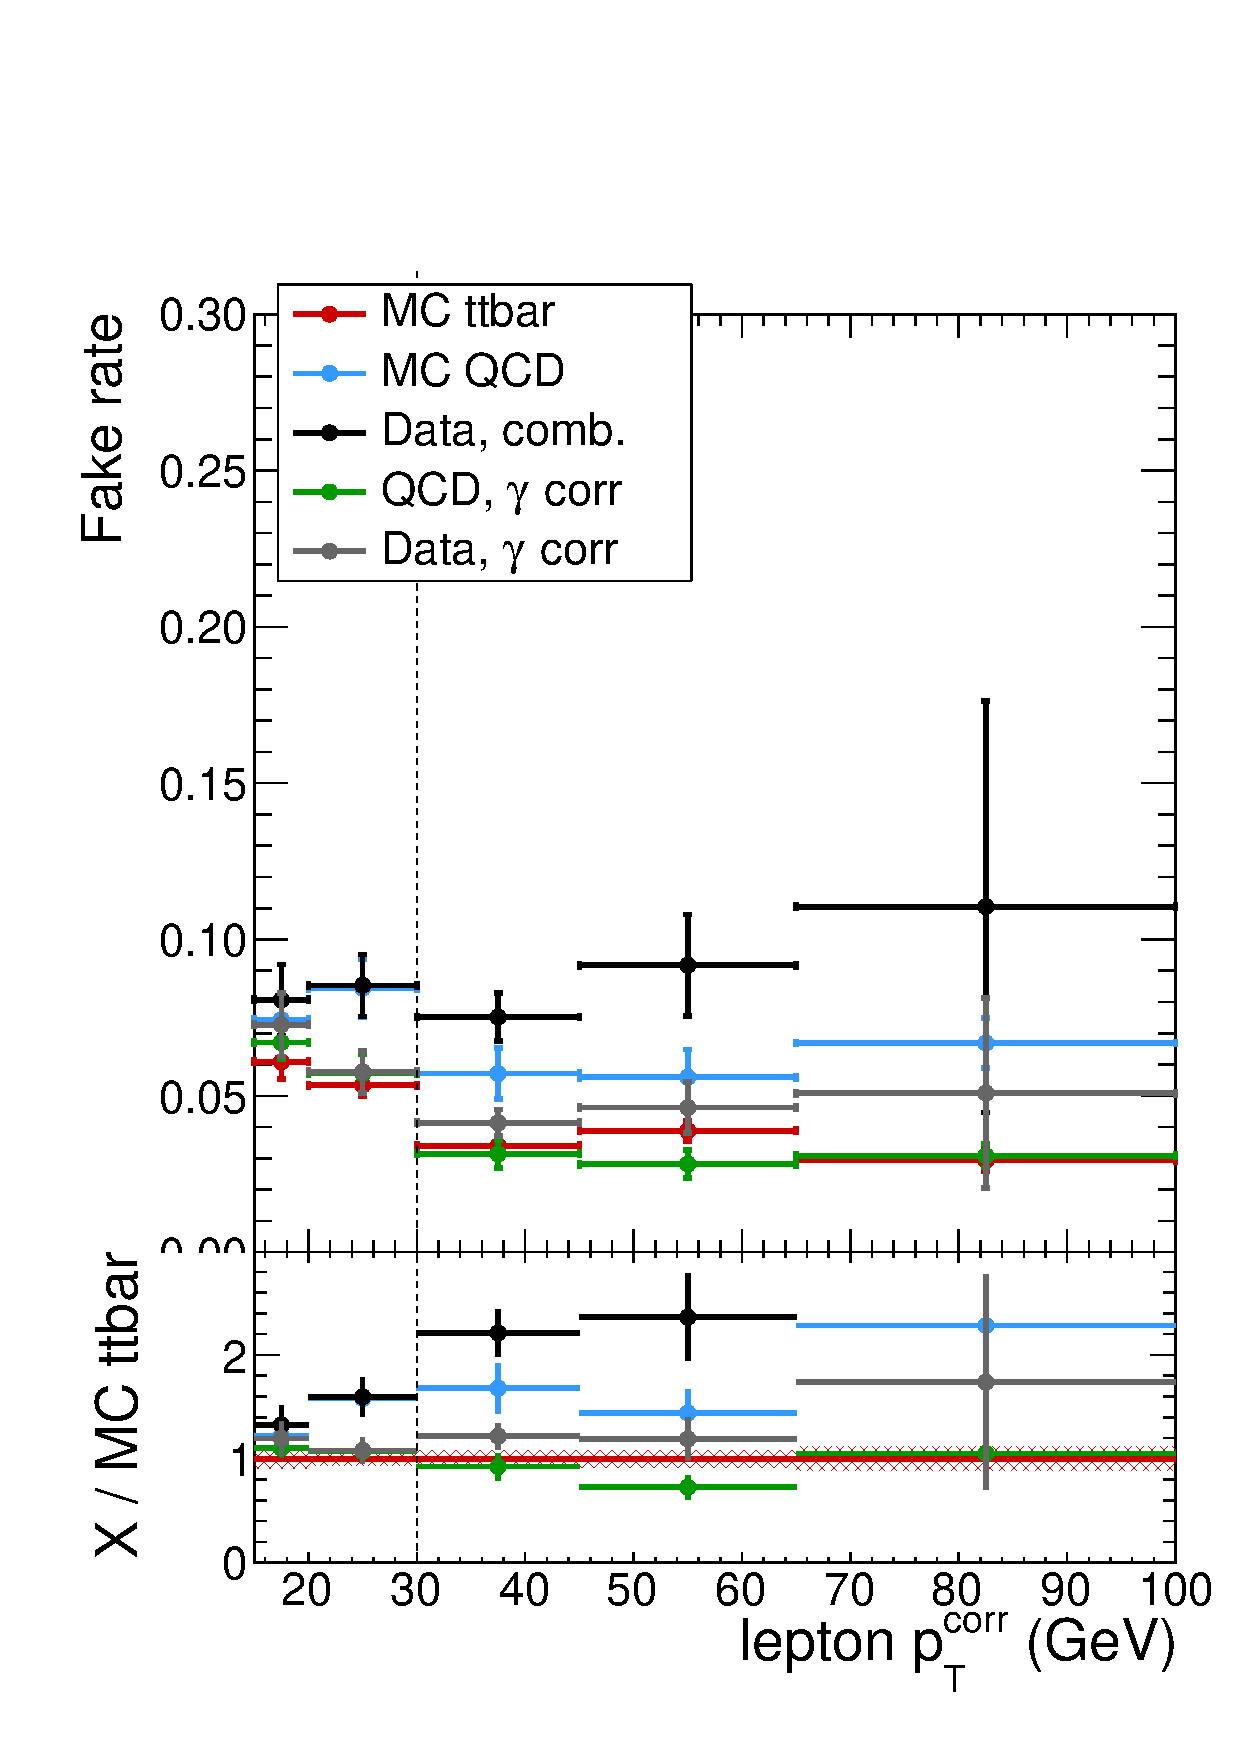
\includegraphics[width=0.35\textwidth]{plots_fakerate/measurement/fr_el_endcap}
    \caption{Summary of the fake rate measurement in events in data, compared with the predictions from simulated events in the measurement region (blue) and from non-prompt leptons in \ttbar (red). Plots in the left column are for muons, those in the right column for electrons; the top row is for the barrel, the bottom for the endcaps. }
\label{fig:frmeas-comb-data}
\end{figure}
